\chapter{Categorie, funtori, trasformazioni naturali}\label{chap_cat_fun_nat}
\section{Categorie}\label{sec_categorie}

Prima di dare una definizione formale di categoria, può essere d'aiuto raccogliere alcuni esempi concreti per orientare chi legge.

La nozione di categoria, che introdurremo in \ref{def_categ}, riuscirà a unificare due strutture matematiche apparentemente molto diverse tra loro:
\index{Monoide}
\begin{definition}\label{prelim_def_monoide}
	Un \emph{monoide} consiste di un insieme \(M\) dotato di
	\begin{itemize}
		\item un elemento \(e\in M\) (spesso denotato anche: \(1_M\) o semplicemente \(1\)), chiamato \emph{elemento neutro}, \emph{unità} o \emph{identità} (si noti che da ciò segue, indirettamente ma immediatamente, che \(M\) è un insieme \emph{non vuoto}),
		\item Un'operazione binaria \(M\times M\to M\), detta \emph{prodotto} o \emph{composizione}, e indicata con \((m,n)\mapsto m\cdot n\) o con simili simboli infissi come \(\star, \centerdot,\bullet\) eccetera,
	\end{itemize}
	che soddisfano le seguenti proprietà:
	\begin{itemize}
		\item \emph{Unitalità}: per ogni \(m\in M\), i prodotti \(m \cdot e\) ed \(e\cdot m\) sono uguali a \(m\);
		\item \emph{Associatività}: per ogni \(m,n,p\in M\), i prodotti \((m\cdot n)\cdot p\) ed \(m\cdot (n\cdot p)\) sono uguali.
	\end{itemize}
\end{definition}
\index{Poset}
\begin{definition}\label{prelim_def_preset}
	Un \emph{insieme preordinato} (o \emph{preordine} o \emph{preset}) consiste di un insieme \(P\) dotato di una operazione binaria \(\le\), solitamente indicata come un simbolo infisso \(x\le y\) per significare che \((x,y)\) è un elemento di \(\le\), che soddisfa le seguenti due proprietà:
	\begin{itemize}
		\item \emph{Riflessività}: per ogni \(x\in P\), si ha \(x\le x\);
		\item \emph{Transitività}: per ogni \(x,y,z\in P\), si ha che
		      \[(x\le y)\;\&\;(y\le z) \quad\implies\quad x\le z\]
	\end{itemize}
	Quando la relazione \(\le\) soddisfa anche la proprietà \emph{antisimmetrica}, cioè è tale per cui
	\[(x\le y)\;\&\;(y\le x) \quad\implies\quad x = y\]
	l'insieme \(P\), o meglio la coppia \((P,\le)\) si dice un insieme \emph{parzialmente ordinato} o \emph{poset}. La relazione \(\le\) in un poset si chiama un \emph{ordine parziale}.
\end{definition}
Dimostreremo in \ref{mon_sonocat} e in \ref{cat_sonopos} rispettivamente che ogni monoide è una categoria, e ogni insieme preordinato (e a fortiori, ogni insieme parzialmente ordinato) è una categoria. (Gli enunciati in questione renderanno più precise queste ultime affermazioni.)
\index{Categoria!--- degli insiemi finiti}
\begin{example}
	Un esempio naturale di categoria nasce considerando la classe \(\ctFin\) di tutti gli insiemi finiti \([n]\defeq \{1,\dots,n\}\) (con la convenzione che \([0]=\varnothing\) sia l'insieme vuoto), e le funzioni \(f : [n] \to [m]\) tra di loro. \`E evidente che non tutte tali funzioni sono componibili: una condizione necessaria --e sufficiente!-- affinché la composizione tra due funzioni \(f : [p] \to [q],g : [m] \to [n]\) tra insiemi finiti sia possibile è che il dominio dell'una coincida con il codominio dell'altra, ovvero che \(q=m\) e che le funzioni si possano `giustapporre' come
	\[\xymatrix{
			[p] \ar[r]^-f & [q] \ar[r]^-g & [r].
		}\]
	La composizione di funzioni \((f,g)\mapsto g\cmp f\) perciò è una operazione che ricorda quella di un monoide (per esempio, essa è associativa quando è definita) ma è appunto un'operazione \emph{parziale}, cioè non definita tra tutte le possibili coppie \((f,g)\) di funzioni tra insiemi finiti; quale che sia la struttura matematica che la classe degli insiemi finiti forma, perciò, essa non può essere un monoide. Un altro motivo per cui \(\ctFin\) non può essere un monoide è che l'identità per la composizione di funzioni non è unica come accade, invece, in ogni monoide: \emph{ogni} insieme finito \([n]\) ha una sua propria funzione identica \(\id_{[n]}\), e se \(f : [m]\to [n]\) con \(m\ne n\), si deve avere che \(f\cmp \id_{[m]}=f=\id_{[n]}\cmp f\) per funzioni identiche formalmente \emph{distinte}, sebbene definite `alla stessa maniera' da \(\lambda x.x : [n]\to [n]\) e \(\lambda y.y : [m]\to [m]\).

	La classe \(\ctFin\) formerà una \emph{categoria}, e per lo stesso motivo faranno altrettanto delle collezioni di oggetti matematici che esibiscono una struttura simile a quella di un monoide, ma sono più generali per motivi simili:
	\begin{itemize}
		\item \index{Categoria!---e di strutture algebriche} la classe \(\bbR\emdash\ctVect\) di tutti gli spazi vettoriali reali della forma \(\bbR^n\) per un \(n\ge 1\) naturale; non tutte le mappe lineari tra spazi vettoriali si possono comporre, e le applicazioni identiche sono tutte distinte; e più in generale,
		\item la classe di tutte le strutture algebriche di un dato tipo (gli insiemi, senza limite alla loro taglia; i gruppi, con gli omomorfismi di gruppo; gli spazi vettoriali, anche di dimensione infinita; gli spazi topologici, con le funzioni continue; eccetera).
	\end{itemize}
\end{example}
Una categoria sarà dunque, in prima approssimazione, una collezione di `oggetti' \(A,B,X,Y,\dots\), legati tra loro da delle relazioni o `funzioni astratte' \(f : X\to Y, g : A\to B\),\dots{} le quali potranno essere composte alla maniera delle funzioni. Questa intuizione è sufficiente per formulare la definizione, a cui deve però prima seguire una precisazione terminologica.
\begin{remark}
	\index{Classe}
	\index{Classe propria|see {Classe}}
	Abbiamo già utilizzato diverse volte la parola `classe': la definizione generale di categoria obbliga a farlo, dal momento che la collezione di tutte le strutture algebriche di un dato tipo è sempre `troppo grande per essere un insieme' (in un senso che formalizzeremo in dettaglio nell'Appendice \ref{fondamenti}); per il momento è sufficiente trattenere l'idea informale che una classe (o \emph{classe propria}) \(\ctC\) è una collezione di elementi che ha tutte le proprietà di un insieme, a parte quella di poter essere misurata da un numero cardinale.

	Ogni volta che è necessario, useremo costruzioni elementari che si possono fare sulle classi come se esse fossero insiemi: per esempio se \(\ctA,\ctB\) sono classi, è lecito costruire la classe prodotto \(\ctA\times\ctB\), e considerare \emph{funzioni tra classi} \(F : \ctA\fun\ctB\), cioè sottoclassi \(F\) del prodotto \(\ctA\times\ctB\) che sono funzionali: per ogni elemento \(A\) della classe \(\ctA\), esiste un unico elemento \(B\in\ctB\) con \((A,B)\in F\), questo elemento si denota \(FA\), e a tutti gli effetti \(F\) si comporta come una funzione. Di nuovo, il linguaggio preciso (il linguaggio \textsf{NBG} della teoria degli insiemi di von Neumann, Bernays e G\"odel) che formalizza queste costruzioni verrà esposto nell'appendice \ref{fondamenti}; questa imprecisione iniziale sarà sempre del tutto innocua, e per il momento invitiamo chi legge a considerare il desiderio di approfondire la cosa solo una inutile distrazione.
\end{remark}
\index{Categoria}
\begin{definition}[Categoria]\label{def_categ}
	Una \emph{categoria} \(\ctC\) consiste dei seguenti dati:
	\begin{enumtag}{c}
		\item\label{c_1} una classe \(\ctC_0\) i cui elementi chiamiamo \emph{oggetti}, di solito indicati con lettere latine maiuscole: \(A\), \(B\), \(X\), \(Y\),\dots
		\item\label{c_2} una classe \(\ctC_1\) i cui elementi chiamiamo \emph{morfismi} o \emph{frecce}, di solito indicati con lettere latine minuscole: \(f,g,h\),\dots, \(u,v,w\)\dots
		\item\label{c_3} Ad ogni morfismo \(f\) corrispondono due oggetti \(\dom{f}\), \(\cod{f}\) chiamati \emph{dominio} e \emph{codominio}. Per denotare il fatto che \(f\) ha dominio \(X\in\ctC_0\) e codominio \(Y\in\ctC_0\), scriveremo \(f\colon X\to Y\), o in \emph{forma diagrammatica},
		\[\begin{tikzcd} X \ar[r, "f"] & Y. \end{tikzcd}\]
		\item\label{c_4} Ogni oggetto \(X\) ha un morfismo distinto \(\id_X\colon X\to X\) chiamato \emph{identità} o \emph{freccia identica}.
		\item\label{c_5} Per ogni coppia di morfismi \(f\colon X\to Y\) e \(g\colon Y\to Z\), cioè tali che \(\cod{f}=\dom{g}\)), è dato un morfismo \(g\circ f:X\to Z\) chiamato \emph{composizione di \(f\) e \(g\)}. Graficamente:
		\[
			\begin{tikzcd}
				X \ar{r}{f}
				\ar[rounded corners,out=-45, in=225]{rr}[swap]{g\cmp f}
				& Y \ar{r}{g} & Z \\
				&&
			\end{tikzcd}
		\]
		(Incidentalmente, osserviamo che \(\dom{g\cmp f}=\dom{f}\) e \(\cod{g\cmp f}=\cod{g}\).)
	\end{enumtag}
	A questi dati, chiediamo di soddisfare le seguenti proprietà:
	\begin{enumtag}{p}
		\item \label{p_1} \emph{Unitalità}: per ogni morfismo \(f:X\to Y\), le composizioni \(f\cmp\id_X\) e \(\id_Y\cmp f\) sono uguali ad \(f\).
		\item \label{p_2} \emph{Associatività}: dati oggetti \(X,Y,Z,W\) e morfismi \(f:X\to Y\), \(g:Y\to Z\) e \(h:Z\to W\), le composizioni \(h\cmp (g\cmp f)\) e \((h\cmp g)\cmp f\) sono uguali.
	\end{enumtag}
\end{definition}
\begin{notation}
	Dati due oggetti \(X\) e \(Y\), indichiamo con \(\Hom{\ctC}(X,Y)\) la classe di morfismi da \(X\) a \(Y\). Altre notazioni, come \(\mathrm{Hom}(X,Y)\) o \(\mathrm{Hom}_\ctC(X,Y)\), sono ugualmente comuni, e motivate dal fatto che le frecce di una categoria astraggono la nozione di \emph{omomorfismo} tra insiemi strutturati (si veda \ref{ex_cat_algebre} e l'esempio \ref{ex_cat_sigma_strutture}).
	% TODO: mettere in una definizione sola "tutte" le categorie di strutture algebriche.
\end{notation}
\begin{remark}\label{cor_def_categ}
	Si osservi che dalla definizione appena data discendono due corollari:
	\begin{itemize}
		\item Le classi \(\Hom{\ctC}(X,Y)\) al variare di \((X,Y)\in\ctC_0\times\ctC_0\) sono tutte disgiunte, perché la corrispondenza \(\ctC_1 \to \ctC_0\times\ctC_0\) che manda \(f\) nella coppia \(\dom{f},\cod{f}\) è una funzione (e allora la sua `fibra' sopra \((X,Y)\) è proprio \(\Hom{\ctC}(X,Y)\), disgiunto da \(\Hom{\ctC}(X',Y')\));
		\item come conseguenza immediata, se \(X\ne X'\) sono oggetti diversi, le identità \(\id_X,\id_{X'}\) sono morfismi diversi: si può cioè pensare la corrispondenza \(X\mapsto \id_X : \ctC_0\to\ctC_1\) come una funzione \emph{iniettiva} tra classi;
		\item la composizione consta di una funzione \emph{parziale}
		      \[\xymatrix{\_\circ\_ : \ctC_1 \times \ctC_1 \ar[r] & \ctC_1}\]
		      il cui dominio è la sotto-classe \(\sum_{XYZ} \{ X \xrightarrow f Y \xrightarrow g Z \}\) dei morfismi \emph{contigui} o componibili. Dato che i vari \(\ctC(X,Y)\) sono a due a due disgiunti, la composizione \(\_\circ\_\) si `decompone' in una classe di funzioni
		      \[\xymatrix{\_\circ_{XZ}^Y\_ : \ctC(Y,Z)\times\ctC(X,Y) \ar[r] & \ctC(X,Z)}\]
		      dove ciascuna manda \(( X \xrightarrow f Y, Y \xrightarrow g Z )\) in \(g\circ f\) (praticamente sempre, si sottintende il dominio particolare di \(\_\circ_{XZ}^Y\_\)).
	\end{itemize}
\end{remark}
\begin{definition}[Categoria piccola, categoria localmente piccola]
	\index{Categoria!--- piccola}
	\index{Categoria!--- loc. piccola}
	Quando la classe \(\ctC_1\) è un insieme, come conseguenza della seconda osservazione fatta, è un insieme anche \(\ctC_0\): in tal caso chiamamo la categoria \(\ctC\) \emph{piccola}: le categorie \(\ctFin\) e \(\bbR\emdash\ctVect\) definite sopra sono piccole, perché abbiamo limitato enormemente la loro classe di oggetti; non abbiamo considerato \emph{tutti} gli insiemi finiti, ma solo quelli della forma \(\{1,\dots,n\}\). Una categoria che non è piccola si dice \emph{grande}, \emph{larga} o simili.

	Invece, \(\ctC\) si dice \emph{localmente piccola} se dati ogni due oggetti \(X\) e \(Y\), la classe \(\Hom{\ctC}(X,Y)\) di morfismi da \(X\) a \(Y\) è un insieme. La categoria di \emph{tutti} gli insiemi finiti non è, strettamente parlando, piccola (perché c'è una classe propria anche solo di insiemi con un singolo elemento: \(\{\varnothing\},\{\{\varnothing\}\}, \{\{\{\varnothing\}\}\}\), eccetera), ma è localmente piccola, perché fissati due insiemi \(X,Y\), la collezione delle funzioni \(f : X\to Y\) è contenuta in \(2^{X\times Y}\), e quest'ultimo è un insieme (per assioma).
\end{definition}
\begin{remark}
	Gli assiomi di categoria non impediscono di costruire `categorie' dove \(\ctC_0\) è un insieme (per esempio, finito) e dove alcuni o tutti \(\Hom{\ctC}(X,Y)\) sono classi; queste costruzioni sono però relativamente innaturali, e non ne parleremo mai. In effetti, non parleremo mai nemmeno di categorie grandi che non sono localmente piccole (ne risentirebbe irrimediabilmente il capitolo 4 del libro, e molti altri risultati). Perciò, da ora in poi adottiamo la convenzione che \emph{categoria} significhi sempre \emph{categoria localmente piccola}. Alternative a questa maniera di ragionare sono possibili, ma non porremo mai una particolare attenzione alla questione.
\end{remark}
Concludiamo con un lemma apparentemente banale, ma che sarà utile in seguito (precisamente, nella dimostrazione di \ref{cat_sonomon}).
\begin{lemma}\label{lem_end_monoide}
	Sia \(\ctC\) una categoria, \(A\in\ctC_0\) un suo oggetto; allora \(M=\Hom{\ctC}(A,A)\) è un monoide, con l'identità \(\id_A\) come elemento neutro e la composizione \(\circ\) come prodotto.
\end{lemma}
\begin{proof}
	La composizione è un'operazione associativa
	\[\begin{tikzcd}
			M\times M \ar[r, "\circ"] & M
		\end{tikzcd}\]
	per \ref{p_2}, e il fatto che \(f\circ \id_A=f=\id_A\circ f\) segue da \ref{p_1}, in \ref{def_categ}.
\end{proof}
Nel resto della sezione raccogliamo alcuni esempi classici di categorie, e nella successiva inizieremo a `costruire categorie nuove dalle vecchie', cioè a definire il \emph{prodotto} \(\ctC\times\ctD\) (si veda \ref{def_cat_prodotto}) e la \emph{somma} \(\ctC+\ctD\) di due categorie date in \ref{def_cat_somma}, le categorie \emph{comma} \(\ctC/X\) e \emph{co-comma} \(X/\ctC\) sopra un oggetto \(X\in\ctC_0\) in \ref{def_cat_cocomma}, la categoria \emph{opposta} \(\ctC^\op\) di \(\ctC\) in \ref{def_cat_opp}, e molte altre.

La dicotomia essenziale che chi legge dovrebbe apprezzare è questa:
\begin{itemize}
	\item le categorie sono strutture ideate per raccogliere una totalità di oggetti matematici di un dato tipo (tutti i gruppi, tutti gli spazi topologici, ecc.) in una classe \(\ctC\) (in \emph{due} classi: gli oggetti e i morfismi) e studiarne le proprietà globali: le categorie (grandi) quindi sono `universi del discorso matematico': questo punto di vista si apprezza particolarmente in \ref{ex_cat_sigma_strutture} e in \ref{ex_cat_top}.
	\item D'altra parte le categorie sono anche delle strutture matematiche a sé stanti, modellate sulla nozione elementare di \emph{multigrafo diretto} (si veda \ref{ex_cat_libera}): le categorie (piccole) quindi sono esse stesse degli oggetti matematici che possiamo studiare alla stregua di ogni altro oggetto matematico (e raccogliere in una loro totalità: ma questo discorso sarà approfondito solo molto più tardi, si veda \ref{ex_cat_cat}).
\end{itemize}
Si può imparare la teoria delle categorie in modo proficuo solo abbracciando \emph{entrambi} questi punti di vista, e ciò perché un dato ambito della matematica si occupa o `vive' in una (o più) categorie. Per esempio, l'algebra lineare studia le categorie \(\bbF\emdash\ctVect\) di spazi vettoriali, eventualmente su diversi campi di base (come \(\bbQ,\bbR,\bbC\), o un campo finito). La topologia generale studia le categorie di \emph{spazi topologici} (e i morfismi funzioni continue), mentre la topologia differenziale si restringe alla categoria i cui oggetti sono \emph{varietà} (e i morfismi funzioni differenziabili), oppure studia particolari categorie di strutture ordinate (perché l'insieme degli aperti di uno spazio topologico \(X\) con una topologia \(\tau \subseteq 2^X\) forma, con le operazioni di unione e intersezione, una struttura algebrica detta \emph{algebra di Heyting}, si veda \cite{Esakia2019}).

D'altra parte l'analisi funzionale studia quegli spazi \emph{vettoriali} (di dimensione infinita) che sono dotati di una \emph{topologia} metrizzabile (e determinata da un filtro di intorni dello zero), ed eventualmente di un prodotto scalare; la teoria della rappresentazione studia certi omomorfismi in un gruppo di matrici, o le proprietà \emph{topologiche-differenziali} di questi gruppi di matrici (il gruppo ortogonale speciale, il gruppo dei quaternioni di norma 1, ecc.). Per comprendere queste strutture è spesso necessario spostarsi di categoria in categoria.

La seconda di queste osservazioni non è meno importante: porterà alla definizione di funtore in \ref{def_funtore} come \emph{omomorfismo tra categorie}, alla definizione di \emph{diagramma} in \ref{def_diagramma} come immagine di una categoria piccola in una categoria, non necessariamente piccola, e alla definizione di trasformazione naturale in \ref{sec_tnat}, vista come \emph{omomorfismo tra funtori}.
\section{Esempi di categorie nella pratica matematica}\label{sec_esempi_cats}
Iniziamo ora a dare degli esempi di categorie piccole: l'esempio più semplice è anche quello più banale.
\index{Categoria!--- vuota}
\begin{example}\label{ex_cat_vuota}
	La categoria vuota \(\ctInit\) non ha oggetti né morfismi. Più formalmente, \(\ctC_0,\ctC_1\) sono le classi vuote, e non è necessario specificare altra struttura per soddisfare (vacuamente) tutti gli assiomi di categoria.
\end{example}
\index{Categoria!--- terminale}
\begin{example}\label{ex_cat_term}
	La categoria terminale \(\ctTerm\) ha un solo oggetto \(\bullet\), e un unico morfismo \(\id_\bullet : \bullet\to\bullet\) che fa da identità. Chiaramente, non si può fare altro che porre \(\id_\bullet\circ\id_\bullet=\id_\bullet\), e tutti gli assiomi di categoria sono soddisfatti.
\end{example}
\index{Categoria!--- discreta}
\`E sempre possibile dotare un insieme \(A\) della topologia discreta (o `massimale'), dove ogni sottoinsieme \(U\) di \(A\) è aperto, e della topologia indiscreta (o `minimale'), dove solo \(\varnothing\) e \(A\) sono aperti. Similmente, esistono due maniere, massimale e minimale, di considerare un insieme\footnote{Riguardo al problema se sia possibile dotare una classe propria della struttura di categoria discreta, la questione \emph{sembra} banale, ma in realtà tutt'altro che semplice da discutere: sebbene non ci sia alcun apparente problema ad assumere l'esistenza di classi proprie discrete, queste spesso vengono proibite \emph{ab imis} assumendo un assioma a parte in aggiunta ai soliti della teoria degli insiemi/classi, detto \emph{principio di Vop\v enka}: questo assioma afferma, precisamente, che non esistono sottoclassi proprie discrete nella classe propria di tutti gli insiemi.} \(A\) una categoria.
\begin{example}\label{ex_cat_discreta}
	Dato un insieme \(A\), la \emph{categoria discreta} su \(A\), denotata \(A^\delta\), ha per oggetti gli elementi \(a\in A\), un unico morfismo identico \(\id_a : a\to a\), e nessun altro. La composizione è forzata a essere definita solamente tra identità, nel modo più ovvio possibile, e tutti gli assiomi di categoria sono ovviamente soddisfatti.
\end{example}
\begin{example}\label{ex_cat_codiscreta}
	Dato un insieme \(A\), la \emph{categoria codiscreta} su \(A\), denotata \(A^\chi\) ha per oggetti gli elementi \(a\in A\), e per ogni coppia di oggetti \(a,a'\in A\), un unico morfismo \(u_{aa'}:a\to a'\), e la composizione è definita da \(u_{a'a''}\circ u_{aa'}=u_{aa''}\) (in particolare, da questo segue che esiste un unico elemento \(\id_a=u_{aa}\in A^\chi(a,a)\)).
\end{example}
Alcune categorie che è spesso utile considerare si rappresentano mediante dei grafi:
\index{Categoria!--- freccia generica}
\begin{example}\label{ex_cat_freccia}
	La categoria `freccia generica' ha due oggetti \(0,1\) e un unico morfismo non identico \(u : 0\to 1\) (che di solito non ha nome). La composizione è forzata a essere definita solamente tra le identità ed \(u\), nell'unico modo ovvio, e tutti gli assiomi di categoria sono banalmente soddisfatti.
\end{example}
\index{Categoria!--- catena generica}
\begin{example}\label{ex_cat_catena}
	Più in generale, la categoria \(\Delta[n]\) detta `catena generica di lunghezza \(n+1\)' è definita come segue:
	\begin{itemize}
		\item gli oggetti di \(\Delta[n]\) sono gli elementi di \(\{0,\dots,n\}\) (ci sono quindi \(n+1\) oggetti, per ogni \(n\ge 1\));\footnote{A volte è utile adottare la convenzione per cui quando \(n=-1\), l'insieme \(\{0,\dots,n\}\) è vuoto, e quindi la categoria `catena di lunghezza \(0\)' è la categoria vuota \(\ctInit\) di \ref{ex_cat_vuota}.}
		\item C'è un unico morfismo \(i\to j\) in \(\Delta[n]\) se e solo se \(i\le j\), di modo che esista un unico morfismo \(i\to i\) (l'identità) per ogni \(i\in\{0,\dots,n\}\), e un unico morfismo \(i\to i+1\) per \(i\in\{0,\dots,n-1\}\); in particolare l'unico morfismo \(i\to j\) è ottenuto dalla composizione
		      \[i\to i+1\to\dots\to j\]
	\end{itemize}
	Le categorie \(\Delta[n]\) per \(=0,1,2,3\) sono rappresentate in figura \ref{fig:le_delta}.
	\begin{figure}[h]
		\begin{center}
			\begin{tikzpicture}
				\node (0) at (0,0) {};
				\fill (0,0) circle (1pt) node[below] {\(0\)};
				%--
				\fill (2,0) circle (1pt) node[below] {\(0\)};
				\node (0') at (2,0) {};
				\fill (3,0) circle (1pt) node[below] {\(1\)};
				\node (1') at (3,0) {};
				\draw[-latex] (0') -- (1');
				%--
				\fill (5,0) circle (1pt) node[below] {\(0\)};
				\node (0'') at (5,0) {};
				\fill (5.5,0.866) circle (1pt) node[above] {\(1\)};
				\node (1'') at (5.5,0.866) {};
				\fill (6,0) circle (1pt) node[below] {\(2\)};
				\node (2'') at (6,0) {};
				\draw[-latex] (0'') -- (1'');
				\draw[-latex] (1'') -- (2'');
				\draw[-latex] (0'') -- (2'');
				%--
				\fill (8,0) circle (1pt) node[below] {\(0\)};
				\node (0'') at (8,0) {};
				\fill (8.5,0.866) circle (1pt) node[above] {\(1\)};
				\node (1'') at (8.5,0.866) {};
				\fill (9,0) circle (1pt) node[below] {\(2\)};
				\node (2'') at (9,0) {};
				\fill (9.5,0.866) circle (1pt) node[above] {\(3\)};
				\node (3'') at (9.5,0.866) {};
				\draw[-latex] (0'') -- (1'');
				\draw[-latex] (1'') -- (2'');
				\draw[-latex] (0'') -- (2'');
				\draw[-latex] (2'') -- (3'');
				\draw[-latex] (1'') -- (3'');
				\draw[-latex] (0'') -- (3'');
			\end{tikzpicture}
		\end{center}
		\caption{Le categorie \(\Delta[0], \dots,\Delta[3]\). Si noti che non abbiamo rappresentato le frecce identiche dei vari oggetti, e che la struttura di categoria che risulta è completamente determinata dalla struttura di grafo diretto. Ovviamente, \(\Delta[0]\) è la categoria terminale di \ref{ex_cat_term}, \(\Delta[1]\) è la freccia generica di \ref{ex_cat_freccia}. La categoria \(\Delta[n]\) spesso si chiama un \(n\)-\emph{simplesso}.}
		\label{fig:le_delta}
	\end{figure}
\end{example}
\index{Categoria!--- doppia freccia generica}
\begin{example}\label{ex_cat_doppiafreccia}
	La categoria `doppia freccia generica' ha due oggetti \(0,1\) ed esattamente due morfismi non identici e paralleli \(s,t : 0\to 1\); anche in questo caso, tali morfismi di solito non hanno nome. La composizione è definita, ancora una volta, nell'unico modo ovvio, chiedendo che \(x\circ \id_0=x=\id_1\circ x\) per \(x\in\{s,t\}\).

	La doppia freccia è la `forma generica' di un grafo diretto (si veda \ref{ex_cat_libera}), dato che una coppia di funzioni \(s,t: X_1 \rightrightarrows X_0\) tra due insiemi consta precisamente di un digrafo che ha \(X_0\) per insieme dei vertici e \(X_1\) per insieme dei lati.
\end{example}
\index{Categoria!--- quadrato generico}
\begin{example}\label{ex_quadcuboncubo}
	La categoria `quadrato generico' \(P[2]\) ha 4 oggetti
	\[\{(00),(10),(01),(11)\} \]
	e un morfismo \((ij)\to(kl)\) se e solo se \(i\le k\) e \(j\le l\); rappresentata graficamente, si tratta della categoria
	\[\begin{tikzcd}
			(00) \ar[r]\ar[d]\ar[dr]& (10)\ar[d] \\
			(01) \ar[r]& (11)
		\end{tikzcd}\]
	La composizione è forzata a essere definita cosicché la composizione \((00)\to (01)\to (11)\) sia uguale alla composizione \((00)\to (10)\to (11)\), e quindi la categoria \(P[2]\) rappresenta la forma generica di un quadrato commutativo.

	Si noti che \(P[2]\) è un insieme ordinato, e precisamente l'insieme dei sottoinsiemi di un insieme con due elementi \(\{a,b\}\); in tal senso \((ij)\) rappresenta la funzione caratteristica \(\chi_U : \{a,b\}\to \{0,1\}\) di un sottoinsieme \(U\subseteq \{a,b\}\), nel senso che ad esempio \((10)=\{a\}, (00)=\varnothing\), eccetera. Si osservi anche che \(P[2]\) è l'insieme parzialmente ordinato \(\{0\le 1\}\times \{0\le 1\}\), dotato dell'\emph{ordine prodotto} (si veda \ref{ord_sonocat} e \ref{cat_sonopos}).

	Quindi possiamo definire induttivamente
	\[P[0] = \Delta[0], \qquad P[n+1] = P[n]\times \Delta[1]\]
	o (equivalentemente, nel senso che questa seconda definizione dà per ogni \(n\ge 0\) un \(P'[n]\) isomorfo a \(P[n]\) come insieme ordinato) \(P'[n] = 2^{\{1,\dots,n\}}\), cosicché \(P[n]\) è il `cubo \(n\)-dimensionale generico': alcune \(P[n]\) per \(n=0,1,2,3\) sono raffigurate in \ref{fig_n_cubo}.
\end{example}
\begin{figure}[h]
	\begin{center}
		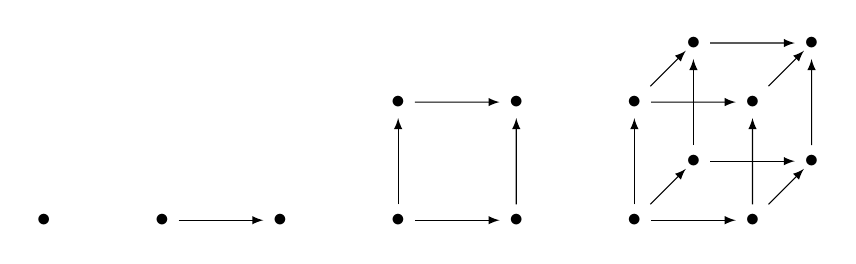
\begin{tikzpicture}[scale=1.5]
			\node (empty) at (-1,0) {\(\bullet\)};
			%
			\node (0) at (0,0) {\(\bullet\)};
			\node (1) at (1,0) {\(\bullet\)};
			\draw[-latex] (0) -- (1);
			\begin{scope}[xshift=2cm]
				\node (00) at (0,0) {\(\bullet\)};
				\node (10) at (1,0) {\(\bullet\)};
				\node (01) at (0,1) {\(\bullet\)};
				\node (11) at (1,1) {\(\bullet\)};
				\draw[-latex] (00) -- (10);
				\draw[-latex] (10) -- (11);
				\draw[-latex] (00) -- (01);
				\draw[-latex] (01) -- (11);
			\end{scope}
			\begin{scope}[xshift=4cm]
				\node (00) at (0,0) {\(\bullet\)};
				\node (10) at (1,0) {\(\bullet\)};
				\node (01) at (0,1) {\(\bullet\)};
				\node (11) at (1,1) {\(\bullet\)};
				\draw[-latex] (00) -- (10);
				\draw[-latex] (10) -- (11);
				\draw[-latex] (00) -- (01);
				\draw[-latex] (01) -- (11);
			\end{scope}
			\begin{scope}[xshift=4.5cm,yshift=.5cm]
				\node (00') at (0,0) {\(\bullet\)};
				\node (10') at (1,0) {\(\bullet\)};
				\node (01') at (0,1) {\(\bullet\)};
				\node (11') at (1,1) {\(\bullet\)};
				\draw[-latex] (00') -- (10');
				\draw[-latex] (10') -- (11');
				\draw[-latex] (00') -- (01');
				\draw[-latex] (01') -- (11');
			\end{scope}
			\draw[-latex, shorten >=-.35pc] (00) -- (00');
			\draw[-latex, shorten >=-.35pc] (01) -- (01');
			\draw[-latex, shorten >=-.35pc] (10) -- (10');
			\draw[-latex, shorten >=-.35pc] (11) -- (11');
		\end{tikzpicture}
	\end{center}
	\caption{Le categorie \(P[n]\) per \(n=0,1,2,3\). La categoria \(P[n]\) si chiama un \(n\)-\emph{cubo}.}
	\label{fig_n_cubo}
\end{figure}
\index{Categoria!--- span generico}
\index{Categoria!--- cospan generico|see {span generico}}
\begin{example}[Span e cospan generici]\label{ex_spancospan}
	La categoria `span generico' \(\Lambda^2_0\) ha tre oggetti \(0,1,2\) e due morfismi non identici. Si raffigura come segue:
	\[\begin{tikzcd}
			1 & 0 \ar[r]\ar[l] & 2
		\end{tikzcd}\]
	La composizione è definita solamente quando almeno una delle due frecce è identica, ed è forzata da questo fatto.

	Dualmente, la categoria `cospan generico' \(\Lambda^2_2\) ha tre oggetti \(0,1,2\) ma i due morfismi non identici escono da \(0\) invece che puntare verso \(2\):
	\[\begin{tikzcd}
			0\ar[r] & 2 & 1\ar[l]
		\end{tikzcd}\]
	Di nuovo, la composizione è definita solamente quando almeno una delle due frecce è identica.

	Si noti che \(\Lambda^2_2\) si ottiene da \(\Delta[2]\) `rimuovendo la freccia \(0\to 1\)', e analogamente \(\Lambda^2_0\) si ottiene rimuovendo la freccia \(1\to 2\).

	Più in generale, sia \(S\) un insieme; la categoria `\(S\)-span generico' \(S^\lhd\) è definita come segue:
	\begin{itemize}
		\item gli oggetti di \(S^\lhd\) sono gli elementi di \(S^+ := S\cup \{-\infty\}\);
		\item esiste un unico morfismo \(f_s : -\infty\to s\), per ogni \(s\in S\).
	\end{itemize}
	La composizione è ancora una volta definita solamente quando almeno una delle due frecce è identica. Questo definisce una categoria in cui da un oggetto chiamato `\(-\infty\)' spiccano tante frecce \(f_s\) quanti sono gli elementi di \(S\).

	Dualmente, definiamo la categoria `\(S\)-cospan generico' \(S^\rhd\) come segue:
	\begin{itemize}
		\item gli oggetti di \(S^\rhd\) sono gli elementi di \(S^+ := S\cup \{+\infty\}\);
		\item esiste un unico morfismo \(f_s : s\to+\infty\), per ogni \(s\in S\).
	\end{itemize}
	La composizione è ancora una volta definita solamente quando almeno una delle due frecce è identica. Questo definisce una categoria in cui verso un oggetto chiamato `\(\infty\)' puntano tante frecce \(f_s\) quanti sono gli elementi di \(S\).

	Si noti che \(\Lambda^2_0=\{1,2\}^\lhd\) e \(\Lambda^2_2=\{0,1\}^\rhd\).
\end{example}
\index{Categoria!--- libera}
Questi ultimi esempi lasciano supporre che \emph{ogni} grafo \(\ctG\), fatto di un insieme di vertici (o `oggetti') \(V\) e di un insieme di lati (o `morfismi') \(E\) generi una categoria \(F\ctG\). \`E effettivamente così, e la seguente costruzione in forma di esempio formalizza questa idea.
\index{Grafo}
\begin{example}\label{ex_cat_libera}
	Dato un grafo (o più propriamente, un \emph{multidigrafo}, ossia una coppia di insiemi \(E,V\) dotati di due funzioni \(s,t : E\rightrightarrows V\) che associano ad ogni \emph{lato} \(e\in E\) una coppia ordinata di \emph{vertici} \(s(e),t(e)\in V\) detti il suo dominio o \emph{source} e il suo codominio o \emph{target}, si veda \ref{ex_cat_grafi}) \(\ctG\) possiamo definire la \emph{categoria libera} \(F\ctG\) su \(\ctG\) come segue:
	\begin{itemize}
		\item gli oggetti di \(F\ctG\) sono esattamente gli elementi di \(V\);
		\item fissati due vertici \(u,v\in V\), i morfismi \(u\to v\) sono l'insieme
		      \[\sum_{n=0}^\infty E(u,x_1)\times\dots\times E(x_n,v)\]
		      di tutte le sequenze ordinate e finite di lati
		      \[ [\tup en;] : u \xto{e_1} x_1 \xto{e_2} x_2\xto{e_3} \dots\xto{e_{n-1}} x_{n-1}\xto{e_n} v\]
		      con la convenzione che se \(u=v\) ed \(n=0\) la sequenza vuota si interpreta come un laccio `banale' \([\;]_u : u\to u\), e usando la notazione, ovvia, \(E(x,y)\subseteq E\) per denotare i lati di source \(x\) e target \(y\).
	\end{itemize}
	La composizione di due sequenze \([\tup fm;]\) e \([\tup en;]\) è data dalla loro \emph{concatenazione}, ossia dalla operazione
	\[[\tup fm;]\circ[\tup en;] = [\tup fm;;\tup en;].\]
	Quando è definita, questa operazione è, evidentemente, associativa, e la sequenza vuota soddisfa la condizione di unitalità \ref{p_1} nella \ref{def_categ}.
\end{example}
Due esempi più elaborati, ma molto `concreti', di categorie dove gli oggetti sono numeri naturali:
\index{Categoria!--- dei circuiti}
\begin{example}[La categoria dei circuiti elettrici]\label{ex_cat_circuiti}
	La categoria \(\ctCirc\) ha
	\begin{itemize}
		\item per oggetti i numeri naturali \(0,1,2,\dots\);
		\item l'insieme dei morfismi \(\ctCirc(m,n)\) consiste dell'insieme delle funzioni \(\bbB^n\to \bbB^m\), dove \(\bbB=\{0,1\}\) è l'insieme dei \emph{Booleani}\footnote{L'insieme \(\bbB\) può essere interpretato come: l'insieme degli interi positivi modulo 2, l'insieme degli stati di un singolo bit di informazione; l'insieme \{sì, no\} delle risposte a una domanda; l'insieme \(\{-1,1\}\) dei \emph{segni} assunti dagli elementi dell'immagine di una funzione reale, l'insieme \{acceso, spento\} degli stati di un interruttore, eccetera.} e \(\bbB^0\defeq \{*\}, \bbB^{n+1}\defeq \bbB^n\times \bbB\) sono i prodotti cartesiani iterati di \(\bbB\) con sé stesso.
	\end{itemize}
	Si noti che ogni funzione Booleana \(f : \bbB^n\to\bbB^m\) risulta dal `prodotto' di \(m\) funzioni Booleane \emph{semplici} \(f_1,\dots,f_m : \bbB^n\to\bbB\), di modo che
	\[f(\tup xn,)=(f_1(\tup xn,),\dots,f_m(\tup xn,))\]
	Tra le funzioni Booleane semplici ci sono certamente le proiezioni canoniche \(\pi_i : \bbB^n\to\bbB :(\tup xn,)\mapsto x_i\), ma anche le mappe diagonali \(\Delta_m:\bbB\to\bbB^m\) definite da
	\[\Delta_m : x\mapsto (x,\dots,x)\quad m\text{ volte}\]
	Sull'insieme dei Booleani è possibile definire le operazioni logiche elementari di disgiunzione, congiunzione e negazione, che rappresentiamo graficamente con i seguenti diagrammi (noti a qualsiasi ingegnere elettronico)
	\[\begin{circuitikz}
			\node[or port, fill=gray!10] (4,0) (or) {\(\lor\)};
			\node[xshift=3cm,and port, fill=gray!10] (0,0) (and) {\(\land\)};
			\node[xshift=5cm,not port, fill=gray!10] (0,0) (not) {\(\lnot\)};
			\node[font=\scriptsize] at (-1,-1) (z1) {\(\_\lor\_ : \bbB^2\to\bbB\)};
			\node[font=\scriptsize] at (2,-1) (z3) {\(\_\land\_ : \bbB^2\to\bbB\)};
			\node[font=\scriptsize] at (5,-1) (z2) {\(\_\lnot : \bbB\to\bbB\)};
		\end{circuitikz}\]
\end{example}
Vale il seguente teorema:
\begin{theorem}
	\Todo{qualcosa che dovrebbe essere nel libro di Walters \cite{Walters1992}, da cui ho preso questo esempio}
\end{theorem}
\index{Categoria!--- dei diagrammi di flusso}
\begin{example}[La categoria dei diagrammi di flusso]\label{ex_cat_flusso}
	La categoria \(\ctFlux\) è definita come segue:
	\begin{itemize}
		\item gli oggetti di \(\ctFlux\) sono i numeri naturali \(0,1,2,\dots\);
		\item l'insieme dei morfismi \(\ctFlux(n,m)\) consiste dell'insieme delle funzioni \(\bbR^n\to \bbR^m\), dove \(\bbR\) consta dell'usuale insieme dei numeri reali, e \(\bbR^n = \bbR\times\dots\times\bbR\) è il prodotto cartesiano iterato di \(\bbR\) con sé stesso.
	\end{itemize}
	\Todo{...}
\end{example}
Proseguiamo con degli esempi di categorie grandi:
\index{Categoria!--- delle relazioni}
\begin{example}[Insiemi e relazioni]\label{ex_cat_rels}
	La categoria \(\ctRel\) ha
	\begin{itemize}
		\item per oggetti gli insiemi, denotati con le lettere \(A,B,C,\dots\);
		\item per morfismi da \(A\) verso \(B\) tutte le \emph{relazioni} \(R\subseteq A\times B\), ossia i sottoinsiemi del prodotto cartesiano \(A\times B\).
	\end{itemize}
	Una relazione \(R\subseteq A\times B\) e una relazione \(S\subseteq B\times C\) si compongono nella relazione \(S\circ R\) definita da
	\[(a,c)\in S\circ R\iff \exists b\in B ((a,b)\in R)\land ((b,c)\in S).\]
	Con questa definizione, si può mostrare che \(T\circ(S\circ R)=(T\circ S)\circ R\) e che la relazione diagonale \(\{(a,a)\mid a\in A\}\subseteq A\times A\) (ovvero la relazione \(a\,\Delta\,a'\iff a=a'\)) funge da elemento identità per la composizione così definita.
\end{example}
Nell'esempio appena fatto, l'ordine in cui si scrivono i fattori di un prodotto cartesiano è importante, perché se \(R : A\to B\) è una relazione, vogliamo che \(A\) ne sia il dominio, e \(B\) il codominio. \`E però vero che gli insiemi \(A\times B\) e \(B\times A\) sono in biiezione canonica, e quindi si potrebbe pensare di definire una categoria \(\ctRel'\) con gli stessi oggetti di \(\ctRel\), ma con morfismi da \(A\) verso \(B\) le relazioni \(R\subseteq B\times A\). In effetti, questa è la categoria opposta \(\ctRel^\op\) di \(\ctRel\) (si veda \ref{def_cat_opp}), e tra \(\ctRel^\op\) e \(\ctRel\) esiste una identificazione canonica.
\index{Categoria!--- degli insiemi}
\index{Categoria!--- degli insiemi finiti|see {--- degli insiemi}}
\begin{example}[Insiemi e funzioni]\label{ex_cat_insiemi}
	La categoria \(\ctSet\) ha
	\begin{itemize}
		\item per oggetti gli insiemi denotati con le lettere \(A,B,C\dots\);
		\item per morfismi da \(A\) vero \(B\) tutte le funzioni \(f : A\to B\), ossia tutte le relazioni \(F\subseteq A\times B\) con la proprietà che per ogni \(a\in A\) esiste un unico \(b\in B\) tale che \((a,b)\in F\) o, più formalmente, \(F\cap(\{a\}\times B)\) è un singoletto; l'elemento \(b\) in questione si denota \(f(a)\) o \(fa\) e l'insieme \(F = \{(a,fa)\mid a\in A\}\) è il \emph{grafico} o \emph{supporto} della funzione. Queste relazioni sono \emph{totali} (perché sono definite sull'intero dominio \(A\)) e \emph{a valore singolo}.
	\end{itemize}
	Due funzioni \(f : A\to B\), \(g : B\to C\) si compongono alla maniera delle relazioni (e la composizione è ancora una funzione, poiché l'intersezione \((G\circ F)\cap (\{a\}\times C)\) consta del singoletto \(\{g(fa)\}\)).

	La relazione diagonale è infine la funzione identica.
\end{example}
Evidentemente, possiamo restringerci a considerare la categoria dei soli insiemi \emph{finiti} (così come la categoria \(\ctFRel\) delle relazioni tra insiemi finiti, che la contiene propriamente). Questo è il primo degli esempi motivanti fatti ad inizio capitolo, e in un senso evidente (che sarà precisato dalla definizione \ref{def_subcat}), \(\ctFRel\) è una \emph{sottocategoria} di \(\ctRel\) (e \(\ctFin\) è una sottocategoria di \(\ctSet\), che a sua volta è una sottocategoria di \(\ctRel\), sebbene in un modo non completamente banale).
\index{Categoria!--- delle matrici}
\begin{example}[Categoria delle matrici in \(\bbF\)]\label{ex_cat_matrici}
	La categoria \(\bbF\emdash\cate{Mat}\) delle \emph{matrici a ingressi in \(\bbF\)} ha
	\begin{itemize}
		\item per oggetti i numeri naturali \(0,1,2,\dots\);
		\item per morfismi \(n\to m\) le matrici con \(m\) righe ed \(n\) colonne a coefficienti in \(\bbF\):
		      \[\bbF\emdash\cate{Mat}(n,m) = M_{m\times n}(\bbF) = \text{Lin}_{\bbF}(\bbF^n,\bbF^m)\]
		      dove \(\bbF^n:=\bbF \times\dots\times\bbF\) è il prodotto cartesiano iterato di \(\bbF\) con sé stesso, e \(\text{Lin}_{\bbF}(\bbF^n,\bbF^m)\) è l'insieme delle funzioni \(\bbF\)-lineari \(\bbF^n\to\bbF^m\).
	\end{itemize}
	La composizione è il prodotto di matrici: se \(A : n\to m\) e \(B : m\to p\) sono matrici di ingressi \((A_{ij}\mid 1\le i\le m,1\le j\le n)\) e \((B_{rs}\mid 1\le r\le p,1\le s\le m)\), la loro composizione \(BA : n\to p\) è la matrice \(BA\in M_{p\times n}(\bbF)\) definita da \((BA)_{ij} = \sum_{k=1}^m B_{ik}A_{kj}\).

	Questa operazione di composizione, come ricorda chiunque abbia studiato l'algebra lineare, è associativa, e la matrice identità \(I_n\in M_{n\times n}(\bbF)\) ne è l'elemento identità.
\end{example}
Questo appena fatto è il secondo degli esempi motivanti fatti ad inizio capitolo.
\index{Categoria!--- di strutture algebriche}
\begin{example}\label{ex_cat_algebre}
	\Todo{Gruppi/monoidi e omomorfismi}
\end{example}
L'\emph{algebra universale} si occupa di generalizzare il concetto di insieme dotato di operazioni, codificando una struttura algebrica in una \emph{funzione di arietà}:\footnote{Le parole \emph{arietà}, così come \emph{nullario} e \emph{unario} e \(n\)-ario (ma non binario, ternario, quaternario, etc.) sono retroformazioni che il lessico matematico ha introdotto a partire dal suffisso latino \emph{-arius}, usato per formare aggettivi a partire da nomi o numerali. Una operazione `\(n\)-aria' accetta \(n\) argomenti a dominio.} innanzitutto, si ricordi che una operazione \(n\)-aria su un insieme \(X\) consta di una funzione \(\tup Xn\times \to X\) dove \(X_i = X\) per ogni \(i=1,\dots,n\).
\index{Categoria!---}
\begin{example}\label{ex_cat_sigma_strutture}
	% \Todo{Omomorfismi per una generica segnatura algebrica}
	Una \emph{segnatura algebrica} consiste di una coppia \((\Omega, a)\) dove \(\Omega\) è un insieme, e \(a : \Omega \to \bfN\) è una funzione detta \emph{funzione di arietà} che associa a ogni elemento \(\omega \in \Omega\) la sua arietà \(a(\omega)\ge 0\). Un \emph{modello} per una segnatura algebrica \((\Omega,a)\) consiste di un insieme \(X\) e di una funzione \(f_\bullet\) che associa a ogni \(\omega\in\Omega\) una operazione \(f_\omega : X^{a(\omega)} \to X\) di arietà \(a(\omega)\).

	Fissata una segnatura algebrica \((\Omega,a)\) possiamo definire la categoria \(\ctMod(\Omega,a)\) dei suoi modelli come segue:
	\begin{itemize}
		\item gli oggetti di \(\ctMod(\Omega,a)\) sono precisamente i modelli \((X,f_\bullet)\) di \((\Omega,a)\);
		\item fissati due modelli \((X,f_\bullet), (Y,g_\bullet)\) un \emph{omomorfismo} di modelli è una funzione \(h : X\to Y\) con la proprietà che per ogni \(\omega\in\Omega\) si abbia l'uguaglianza
		      \[h(f_\omega(\tup x{a(\omega)},)) = g_\omega(\tup {hx}{a(\omega)},)\]
		      o in termini diagrammatici:
		      \[bla\]
	\end{itemize}
\end{example}
\`E un esercizio tedioso nella manipolazione delle tuple ordinate, ora, dimostrare che gli assiomi di categoria sono tutti soddisfatti. Un esercizio analogamente tedioso è di trovare segnature algebriche opportune che esprimono le categorie dei gruppi, dei monoidi, degli anelli e degli spazi vettoriali ecc. come esempi particolari di categorie di modelli di una segnatura algebrica. (Tedioso, e a volte non proprio banale: ad esempio, come si descrivono le operazioni di moltiplicazione per scalare in uno spazio vettoriale usando la definizione di segnatura algebrica?)
\begin{example}[Categoria dei grafi]\label{ex_cat_grafi}\index{Categoria!--- dei grafi}
	\Todo{}
\end{example}
\index{Categoria!--- di insiemi ordinati}
\index{Preordine}
\begin{example}\label{ex_cat_ordini}
	Si ricordi da \ref{prelim_def_preset} che un \emph{insieme preordinato} è un insieme \(P\) dotato di una relazione riflessiva e transitiva \(\le\); una funzione \(f  : (P,\le)\to (Q,\preceq)\) si dice \emph{monotòna} o si dice che \(f\) \emph{preserva l'ordine} se vale
	\[\forall x,y(x\le y\Rightarrow fx\le fy).\]

	La categoria \(\ctPOrd\) ha per oggetti e morfismi gli insiemi preordinati e le funzioni monotòne. Chiaramente, l'identità \(\id_P : (P,\le)\to (P,\le)\) è una funzione monotòna, e la composizione di due funzioni monotòne resta monotòna.

	\`E tuttavia importante che l'ordine su \(P\) sia \emph{lo stesso} affinché l'identità sia monotòna: infatti, ogni insieme \(P\) può essere dotato dell'ordine \emph{banale} (dove \(x \mathrel{\le^\delta} y\) se e solo se \(x=y\)) e dell'ordine \emph{caotico} (dove \(x\mathrel{\le^\chi} y\) per ogni \(x,y\in P\)). Se \(P\) ha almeno tre elementi, la funzione identica \((P,\le^\chi)\to (P,\le^\delta)\) non è, chiaramente, monotòna.
\end{example}
\index{Ordine parziale}
\begin{remark}[po, wo e to]\label{po_wo_to}
	Una sottoclasse importante di preordini sono quelli dove \(\le\) è una relazione antisimmetrica; in tal caso il preordine \((P,\le)\) si dice un \emph{insieme parzialmente ordinato} o \emph{poset}. La categoria \(\ctPos\) ha per oggetti i poset e per morfismi le stesse funzioni monotòne di \ref{ex_cat_ordini}.

	Un'altra sottocategoria importante di \(\ctPOrd\) è quella degli insiemi \emph{totalmente ordinati} o \emph{toset}, dove tutti gli elementi sono confrontabili tra loro:
	\[\forall x,y\in P((x\le y)\lor (y\le x)).\]
	Da ultimo, una ulteriore sottocategoria importante di \(\ctPOrd\) è quella degli insiemi \emph{bene ordinati} o \emph{woset}, dove ogni sottoinsieme non vuoto ammette un elemento minimo.
\end{remark}
\index{Categoria!--- degli ordinali}
\begin{example}\label{ex_cat_ordinali}
	Un insieme si dice \emph{transitivo} se una qualsiasi delle seguenti condizioni equivalenti è soddisfatta:
	\begin{itemize}
		\item \(x\in X\Rightarrow x\subseteq X\);
		\item \(X\subseteq 2^X\);
		\item \(\bigcup X\subseteq X\).
	\end{itemize}
	Un insieme è un \emph{ordinale} se è transitivo e se ogni sottoinsieme non vuoto \(S\subseteq X\) ammette un elemento \(\in\)-minimo, cioè se \(X\) è bene ordinato dalla relazione \(\in\).

	La categoria \(\ctOrd\) ha per oggetti gli ordinali e per morfismi \(X\to Y\) le funzioni monotòne.
\end{example}
L'importanza della categoria degli ordinali sarà più evidente quando in \ref{sec_funtori} introdurremo la definizione di funtore. Per il momento, ci limitiamo ad alcune osservazioni.
\begin{remark}
	Se \([n]=\{1,\dots,n\}\) è un insieme finito, l'ordinamento \(\{1<2<\dots<n\}\) lo rende un woset nel senso di \ref{po_wo_to}, e quindi \(\Delta[n]\) è in maniera naturale un oggetto di \(\ctPos\), ma anche di \(\ctOrd\); insieme alle funzioni monotòne tra questi insiemi finiti, ciò identifica la sottocategoria di \(\ctOrd\) generata da tutte le catene generiche \(\Delta[n]\) di \ref{ex_cat_catena} con la sottocategoria \(\ctFOrd\) di tutti gli ordinali finiti
\end{remark}
\begin{remark}
	Senza un assioma dedicato a tale scopo, non si possono generare ordinali più grandi di quelli finiti; al contrario, assumendo che esista almeno un insieme \emph{induttivo} \(N\) (cioè tale che, se \(x\in N\), allora \(x^+:=x\cup\{x\}\in N\)), possiamo `accedere' a ordinali più grandi, e da qui generarne di \emph{molto} grandi (abbastanza da far sì che la categoria \(\ctOrd\) abbia una classe propria di oggetti).

	Questa è una maniera un po' semplificata di introdurre l'ordinale \(\omega\) ottenuto come `limite' di tutti gli ordinali finiti \([n]\): rinviamo chi legge a un corso di logica elementare per approfondire la questione in modo più tecnico, e ci limitiamo a osservare che la dicotomia importante nella definizione di un numero ordinale è la seguente: un ordinale \(\alpha\in\ctOrd_0\) può essere di due tipi: un \emph{successore}, se esiste \(\beta\) tale che \(\alpha=\beta^+\), e un ordinale \emph{limite} se, invece, \(\alpha=\bigcup\alpha=\sup\{\gamma\mid \gamma < \alpha\}\).
\end{remark}
\begin{remark}
	L'importanza degli ordinali risiede nella possibilità di dare \emph{definizioni induttive} (per induzione, finita o transfinita): se \(\ctC\) è una classe, una funzione di classe \(H : \ctOrd_0\to\ctC\) spesso è univocamente determinata dalla specifica
	\begin{itemize}
		\item di un elemento \(H(0)\in\ctC\) detto base dell'induzione;
		\item di una maniera di calcolare \(H(x+1)=H(x^+)\) in termini degli elementi precedenti \(H(0), H(1),\dots,H(x)\); questo è il \emph{passo induttivo} della costruzione;
		\item di una maniera di calcolare il `passo limite' dell'induzione, \(H(\lambda)\), in termini di \(H(\gamma)\) per \(\gamma < \lambda\).
	\end{itemize}
	Un esempio particolare si apprezzerà con la definizione di funtore, dato che una maniera di formalizzare le successioni
	\[\begin{tikzcd}
			A_0 \ar[r] & A_1 \ar[r] & A_2 \ar[r] & \dots \ar[r] & A_\alpha
		\end{tikzcd}\]
	\emph{eventualmente infinite} di morfismi contigui in una categoria \(\ctC\) sarà esattamente come un funtore \(\ctOrd_{\le\lambda}\funto \ctC\).
\end{remark}
\index{Categoria!--- di spazi topologici}
\begin{example}\label{ex_cat_top}
	\Todo{Spazi e funzioni continue}
\end{example}
\index{Categoria!--- di funzioni parziali}
\begin{example}\label{ex_cat_pfun}
	\Todo{Insiemi e funzioni parziali}
\end{example}
\index{Categoria!--- di insiemi puntati}
\begin{example}\label{ex_cat_puntati}
	\Todo{Insiemi puntati}
\end{example}
\index{Categoria!--- di azioni di gruppo}
\begin{example}\label{ex_cat_g_insiemi}
	\Todo{Azioni di \(G\)}
\end{example}
\index{Categoria!--- di `stream'}
\begin{example}\label{example_streams}
	La categoria \(\cate{Stream}\) ha
	\begin{itemize}
		\item per oggetti gli insiemi \(A,B,C\dots\)
		\item per morfismi \(f : A\pto B\) le funzioni della forma
		      \[\longmor{f : \sum_{n=1}^\infty A^n}{B}\]
		      dove il dominio \(A^+=\sum_{n=1}^\infty A^n\) è l'insieme delle \emph{liste non vuote} di elementi di \(A\), cioè l'insieme \(A + (A\times A) + (A\times A\times A) + \dots\) i cui elementi sono sequenze ordinate della forma \((\tup an,)\) per \(n\ge 1\) e \(a_i\in A\) per ogni \(i=1,\dots,n\).\footnote{In termini più formali, \(A^+\) è il \emph{semigruppo libero} generato dall'insieme \(A\), un `semigruppo' essendo un insieme dotato di una operazione binaria associativa.}
	\end{itemize}
	L'intuizione dietro questa definizione è che un morfismo \(f \in \Hom{\cate{Stream}}(A,B)\) consiste di un `algoritmo' che data una lista non vuota di input \((\tup an,)\) calcola un output \(f(\tup an,)\in B\) (che chiaramente può dipendere anche da \(n\)), per ogni \(n\ge 1\).

	Le identità sono le funzioni \(\sum_{n=1} A^n\to A\) definite mandando \((\tup an,)\) in \(a_n\); la composizione è data, se \(f : A\pto B\) e \(g : B\pto C\) dalla regola \(g\circ f : A\pto C\)
	\[(\tup an,)\longmapsto g\big(f(a_1),f(a_1,a_2),\dots f(\tup a{n-1},),f(\tup an,)\big).\]
	Ovvero, la composizione \(g\circ f\) calcola l'output che la funzione \(g\) genera a partire dagli input \(f(a_1),f(a_1,a_2),\dots f(\tup a{n-1},),f(\tup an,)\).
\end{example}
\begin{example}[La categoria degli insiemi dimensionati]\label{example_dimensionati}
	La categoria \(\cate{dSet}\) degli \emph{insiemi con unità di misura} o `insiemi dimensionati' ha
	\begin{itemize}
		\item per oggetti le funzioni suriettive \(d : A\to D\) verso un insieme \(D\) che svolge il ruolo di insieme delle unità di misura con cui gli elementi di \(A\) sono etichettati; se, ad esempio \(D := \{m,s,kg\}\), gli elementi di \(d^{-1}(m)\) sono le `lunghezze' (cioè si misurano in metri), gli elementi di \(d^{-1}(s)\) sono i tempi, eccetera.
		\item dati due insiemi dimensionati \((d : A\to D)\) e \((d', B\to D')\), un morfismo tra di loro consiste di una coppia di funzioni \(u,v\) che fanno commutare il seguente quadrato:
		      \[\begin{tikzcd}
				      A\ar[r, "u"]\ar[d,"d"'] & B \ar[d, "d'"]\\
				      D \ar[r, "v"']& D'
			      \end{tikzcd}\]
	\end{itemize}
\end{example}
Veniamo ora a degli esempi più astratti e chiudiamo il cerchio su quelli che hanno motivato la definizione di categoria all'inizio.

Un'ottima intuizione sulla definizione \ref{def_categ} è che in qualsiasi circostanza dove una classe di strutture possiede una nozione ovvia di omomorfismo che preserva la specifica di quella struttura, e tale che
\begin{itemize}
	\item l'identità è un omomorfismo;
	\item la composizione di due omomorfismi è ancora un omomorfismo;
\end{itemize}
si riesce a definire la classe degli oggetti e dei morfismi di una categoria. Gli esempi di strutture algebriche sono tutti di questo tipo, ovviamente; ne esistono altri, che non riguardano le operazioni algebriche: per esempio, la composizione di due mappe monotòne è monotòna, e la composizione di due mappe \emph{proprie} tra spazi di Hausdorff è ancora una mappa propria.

Fin qui, l'osservazione che le strutture matematiche di un dato tipo, con la definizione appropriata di omomorfismo, formino una categoria, è nient'altro che una banalità della prassi matematica. Una osservazione decisamente meno banale è che alcune delle strutture basilari della pratica matematica sono \emph{esse stesse} delle categorie.

In più, questo modo di intendere la definizione oscura un'altra idea importante, perché l'esempio \ref{ex_cat_sigma_strutture} potrebbe far sospettare che gli oggetti di una categori siano, alla fin fine, sempre insiemi dotati di strutture ulteriori (per esempio, operazioni o relazioni), e i morfismi funzioni che preservano queste strutture.

Invece, le categorie che hanno questa proprietà si dicono \emph{concrete}, ed esistono esempi di categorie non concrete (sebbene essi siano piuttosto ardui da definire); chi legge può consultare \cite{Freyd1973,Kuera1971} per maggiori informazioni.
\index{Relazione di equivalenza}
\begin{example}\label{ex_cat_rel_equiv}
	Un insieme dotato di una relazione di equivalenza si può vedere come una particolare categoria. Consideriamo un insieme \(X\) dotato di una relazione di equivalenza indicata con il simbolo \(\sim\).
	Definiamo la seguente categoria \(\ctB(X,\sim)\):
	\begin{itemize}
		\item Gli oggetti di \(\ctB(X,\sim)\) sono gli elementi di \(X\);
		\item Esiste un unico morfismo \(x\to y\) se e solo se \(x\sim y\) (e allora esiste anche un unico morfismo \(y\to x\) come conseguenza del fatto che \(\sim\) è simmetrica).
	\end{itemize}
	Per ogni oggetto \(x\), l'identità è l'unico morfismo \(x\to x\) dato dal fatto che la relazione è riflessiva (\(x\sim x\)).
	La composizione è data dalla transitività: se abbiamo morfismi \(x\to y\) e \(y\to z\) significa, in particolare, che \(x\sim y\) e \(y\sim z\). Per transitività, \(x\sim z\), e quindi c'è un unico morfismo \(x\to z\), che possiamo definire come composizione.

	Gli assiomi di unitalità e associatività sono automaticamente soddisfatti: per esempio, la composizione \((w\to x\to y)\to z\) e la composizione \(w\to (x\to y\to z)\) coincidono, constando dell'unico morfismo \(w\to z\).
\end{example}
Quelle della forma \(\ctB(X,\sim)\) per qualche insieme \(X\) e relazione di equivalenza \(\sim\) sono un primo esempio elementare di categoria in cui gli oggetti non sono insiemi strutturati, ma non è quello più semplice possibile: la proprietà di simmetria di \(\sim\) non è essenziale per ottenere una categoria.

Consideriamo ora i seguenti esempi di categorie simili (che raccogliamo in dei teoremi, di cui diamo una dimostrazione completa, perché questi esempi sono pedagogicamente rilevanti).
\index{Categoria!--- da una relazione}
\begin{examples}\label{ord_sonocat}
	Ogni relazione d'ordine \((X,\le)\) forma una categoria, ancora una volta con un unico morfismo \(x\to y\) se e solo se \(x\le y\). Come nel caso delle relazioni di equivalenza, gli oggetti di \(\ctP(X,\le)\) sono gli elementi di \(X\), le identità sono date dalla proprietà riflessiva \(x\le x\) e la composizione dalla proprietà transitiva. Ciò è sufficiente a soddisfare tutti gli assiomi di categoria.

	Più in generale, un \emph{preordine} è una relazione riflessiva e transitiva, ma non necessariamente simmetrica o antisimmetrica. Ogni preordine si può vedere come una categoria alla stessa maniera di prima.
\end{examples}
\begin{remark}
	Due osservazioni sono a questo punto importanti:
	\begin{itemize}
		\item è facile fraintendere la definizione appena data, o perlomeno esserne confusi, perché la definizione di categoria data in \ref{def_categ} chiede che esista un \emph{insieme} di morfismi \(x\to y\) tra due oggetti \(x,y\) di \(\ctP(X,\le)\).

		      Qual è quindi l'insieme di morfismi tra \(x\) e \(y\)? La risposta è che, in questo caso, tra due morfismi esiste una \emph{proposizione}, precisamente quella che asserisce se \(x\le y\) o meno. Il problema di rendere questa proposizione un insieme si risolve così: diciamo che \(\ctP(X,\le)\) è un insieme con un singolo elemento (lo chiamiamo \([x\le y]\)) se e solo se \(x\le y\) `è vera', ed è l'insieme vuoto altrimenti. In questo modo, dobbiamo definire una regola di composizione tra l'elemento \([x\le y]\) e l'elemento \([y\le z]\): questo non può che essere l'elemento \([x\le z]\), e a questo punto lasciamo i dettagli (tediosi) da scrivere a chi legge.
		\item \`E fondamentale non rimanere confusi da un altro dettaglio: in base a \ref{ex_cat_ordini} esiste una categoria i cui oggetti sono gli insiemi ordinati \((X,\le)\) e i cui morfismi sono le funzioni monotòne. In base a \ref{ord_sonocat}, \emph{ogni} insieme ordinato \((X,\le)\) è \emph{esso stesso} una categoria i cui oggetti sono gli elementi di \(X\). Queste due asserzioni sono molto diverse tra loro; sarà la definizione \ref{ex_cat_cat} a rendere preciso in che senso \(\ctPos\) è una `categoria di categorie'.
	\end{itemize}
\end{remark}
Occupiamoci ora di dimostrare che una categoria dove tra due oggetti esiste al più un morfismo è \emph{precisamente} un insieme (pre)ordinato.
\begin{theorem}\label{cat_sonopos}
	% \Todo{rovescio: una categoria dove ogni hom-set ha al piu un elemento è un preset}
	Sia \(\ctC\) una categoria, con la proprietà che \(\ctC(X,Y)\) ha al più un elemento. Allora, la relazione
	\[X\le Y \iff \ctC(X,Y) \text{ non è vuoto}\]
	definisce una struttura di insieme preordinato su \(\ctC_0\).
\end{theorem}
\begin{proof}
	La relazione così definita è
	\begin{itemize}
		\item riflessiva, perché \(\ctC(X,X)\) contiene l'identità (e solo l'identità);
		\item transitiva, perché se \(\ctC(X,Y), \ctC(Y,Z)\) non sono vuoti, la composizione è definita come in \ref{cor_def_categ} e quindi esiste esattamente un elemento in \(\ctC(X,Z)\).
	\end{itemize}
\end{proof}
\index{Categoria!--- da un monoide}
Esiste un altro esempio di questo fatto (alcune strutture matematiche sono esse stesse una categoria): infatti, ogni monoide si può vedere come una categoria che ha un solo oggetto. Questi sono precisamente gli esempi iniziali con cui abbiamo motivato la definizione \ref{def_categ}.
\begin{theorem}\label{mon_sonocat}
	Dato un monoide \((M,\cdot,1)\), definiamo la seguente categoria, che indichiamo con \(\ctB M\).\footnote{A volte la categoria definita in questo modo si indica con \(\ctB(M,\cdot)\), a volte (quando l'operazione su \(M\) è ovvia dal contesto) semplicemente con \(\ctB M\).}
	\begin{itemize}
		\item La categoria \(\ctB M\) ha un unico oggetto, che indichiamo con \(\star\);\footnote{La notazione è volta a suggerire che precisare questo elemento non sarà mai importante (una scelta canonica, ma che potrebbe causare confusione, è fissare \(\ctB M_0 := \{M\}\), insieme che ovviamente \emph{non} è \(M\)).}
		\item La categoria \(\ctB M\) ha un morfismo \(m:\star\to\star\) per ogni elemento \(m\in M\); l'unico hom-insieme che dobbiamo specificare, \(\Hom{\ctB M}(\star,\star)\), è cioè uguale a \(M\), e in particolare, l'identità \(\id_\star\) è l'elemento neutro \(1\in M\);
		\item La composizione di morfismi
		      \[\longmor{\Hom{\ctB M}(\star,\star)\times \Hom{\ctB M}(\star,\star)}{\Hom{\ctB M}(\star,\star)}\]
		      è data dal prodotto \(M\times M\to M\).
	\end{itemize}
\end{theorem}
Chi legge dovrebbe ora riflettere su questa frase finché essa non appare perfettamente evidente: nell'esempio appena fatto, gli assiomi di categoria sono \emph{precisamente} gli assiomi che definiscono un monoide.

Di converso, i monoidi sono esattamente tutte e sole le categorie che hanno un solo oggetto:
\begin{theorem}\label{cat_sonomon}
	Data una categoria \(\ctC\) tale che \(\ctC_0\) abbia un singolo elemento \(\star\), l'insieme \(\ctC_1 = \Hom{\ctC}(\star,\star)\) è un monoide come conseguenza di \ref{lem_end_monoide}.
\end{theorem}
% \begin{example}\label{ex_cat_mon}
% 	In un monoide, a differenza di una categoria generica, possiamo sempre comporre due morfismi \(m\) e \(n\): questo è garantito dal fatto che siccome c'è un solo oggetto, il dominio e il codominio di \(m\) ed \(n\) sono necessariamente uguali.
%
% 	Viceversa, data una categoria localmente piccola con un solo oggetto (indichiamolo ancora con questo simbolo, \(\bullet\)), l'insieme di morfismi \(\bullet\to\bullet\) ha una struttura di monoide con l'elemento neutro dato dall'identità, e il prodotto dato dalla composizione.
%
% 	L'unitalità e l'associatività del monoide e della categoria si corrispondono.
% \end{example}
\begin{corollary}\label{cor_cat_mon}
	In particolare, un gruppo \((G,\cdot,1)\) si può ugalmente vedere come la categoria \(\ctB G\) ad esso associata, che ha un solo oggetto e \(G\) come insieme di morfismi. In maniera concisa (ma anche ora, chi legge dovrebbe fermarsi a riflettere finché questa frase non risulta perfettamente evidente) un monoide è una categoria con un singolo oggetto, e un gruppo è un gruppoide (come in \ref{def_gruppoide}) con un singolo oggetto.
\end{corollary}
\begin{remark}
	Del resto, una categoria con un solo oggetto non `è' un monoide, ma lo definisce naturalmente; e un monoide non `è' la categoria \(\ctB M\), ma la definisce naturalmente (e qualcosa di simile si può dire per gli insiemi ordinati). In altre parole, eliminare la distinzione tra \(M\) e \(\ctB M\) non segue da una tautologia, ma è una \emph{identità informativa} (intesa come in `Senso e significato` di Frege) che non è \emph{strettamente} una identità ma una \emph{identificazione}: \(M\mapsto \ctB M\) e \(\ctC\mapsto \ctC_1\) sono, a patto che \(\ctC_0\) abbia un solo elemento, corrispondenze inverse una dell'altra, nel senso che \((\ctB M)_1 = M\) e che \(\ctB(\ctC_1) = \ctC\).
	%Dato un oggetto \(X\) di una categoria, un morfismo da \(X\) a \(X\) si chiama anche \emph{endomorfismo}. In un monoide, tutti i morfismi sono endomorfismi.
\end{remark}
% \begin{remark}
% 	Abbiamo visto che i gruppi sono gli oggetti della categoria \(\ctGrp\), ma anche che ogni gruppo si può a sua volta vedere come una categoria (con un solo oggetto). Entrambe le prospettive sono valide, e ce ne sono altre ancora.
% 	Allo stesso modo, gli ordini parziali sono categorie, ma si possono anche vedere come oggetti della categoria \(\ctPos\), dove i morfismi sono le funzioni monotone.
% 	Spesso, in teoria delle categorie, la stessa struttura matematica può apparire in modi diversi in contesti diversi, e questa varietà di prospettive è uno dei motivi per cui le categorie sono così versatili.
% \end{remark}
\subsubsection*{Esercizi}
\begin{enumerate}
	\item Un \emph{grafo diretto} (chiamato anche \emph{digrafo}) è un insieme \(V\), i cui elementi chiamiamo \emph{vertici}, e una relazione \(E\subseteq V\times V\), i cui elementi chiamiamo \emph{spigoli}. Diciamo che \(x\) è \emph{adiacente} a \(y\) se esiste uno spigolo \((x,y)\in E\). Un \emph{omomorfismo di grafi diretti} \(f:(V,E)\to (V',E')\) è una funzione \(f:V\to V'\) tale che se \(x\) è adiacente a \(y\), allora \(f(x)\) è adiacente a \(f(y)\). Dimostra che i grafi diretti e i loro omomorfismi formano una categoria.
	\item Un \emph{multigrafo diretto} (chiamato anche \emph{multidigrafo}) è definito similmente a un grafo diretto, ma può avere diversi spigoli tra gli stessi due vertici. Un multidigrafo consiste di un insieme \(V\) (i \emph{vertici}), e un insieme \(E\) (gli \emph{spigoli}), con due funzioni \(d_-,d_+:E\to V\), che associano un ``dominio'' e un ``codominio'' ad ogni spigolo. Un \emph{omomorfismo di multigrafi diretti} \((V,E)\to (V',E')\) consiste di una funzione \(f_0:V\to V'\) tra i vertici, e una funzione \(f_1:E\to E'\) tra gli spigoli, compatibili con le mappe \(d_-,d_+\) nel seguente modo:
	      \[
		      d_-(f_1(e)) = f_0(d_-(e)) ,\qquad d_+(f_1(e)) = f_0(d_+(e)) .
	      \]
	      Dimostra che \(f_1:E\to E'\) associa a uno spigolo tra \(x\) e \(y\) uno spigolo tra \(f_0(x)\) e \(f_0(y)\).
	\item Dimostra che i multigrafi diretti e i loro omomorfismi formano una categoria.
	\item Una categoria piccola si può vedere come un multigrafo con identità e composizione: riscrivi la definizione di categoria (piccola) in termini di multigrafi.  In che modo questa costruzione generalizza la definizione di monoide (come insieme con identità e composizione)?
	\item Dimostrare che  se \((P,\le)\) è un insieme bene ordinato, ed \(f : P\to P\) è una funzione monotòna, allora \(a\le fa\) per ogni \(a\in P\) (cioè ogni endofunzione di un woset è \emph{espansiva}); dimostrare che l'unica biiezione monotòna di un woset è l'identità; più in generale, se esiste un isomorfismo d'ordine \(f : P\to Q\) tra due woset, allora esso è unico.
\end{enumerate}
\section{Operazioni tra categorie}\label{sec_operazioni}

\Todo{categoria prodotto, categoria somma, categoria opposta,}
\index{Categoria!sotto---}
\begin{definition}\label{def_subcat}
	\Todo{sottocategoria}
\end{definition}
\begin{definition}\label{def_cat_prodotto}
	\Todo{Categoria prodotto}
\end{definition}
\index{Categoria!--- somma}
\begin{definition}\label{def_cat_somma}
	\Todo{Categoria somma}
\end{definition}
\index{Categoria!--- comma}
\index{Categoria!--- opposta}
\begin{definition}\label{def_cat_opp}
	\Todo{Categoria opposta}
\end{definition}
\begin{remark}
	Diciamo che una categoria \(\ctC\) è \emph{autoduale} se \(\ctC=\ctC^\op\).

	Chiaramente, la categoria vuota \(\ctInit\) è autoduale (ossia \(\ctInit^\op=\ctInit\)) e altrettanto è vero per la categoria terminale \(\ctTerm\) e per la categoria discreta \(A^\delta\) di \ref{ex_cat_discreta}.

	La categoria \(\Delta[n]\) di \ref{ex_cat_catena} si identifica alla sua opposta mediante la funzione \(j\mapsto n-j\), la quale inverte l'ordine, e risulta quindi un anti-isomorfismo tra l'insieme ordinato \(\Delta[n]=(\{1,\dots,n\},\le)\) e l'insieme ordinato \(\Delta[n]^\op = (\{1,\dots,n\},\ge)\).
	\Todo{Esercizio: la categoria codiscreta di \ref{ex_cat_codiscreta} si identifica alla sua opposta mediante...}

	Le categorie `span generico' e `cospan generico' sono opposte l'una dell'altra, e altrettanto è vero per le categorie \(S^\lhd\) e \(S^\rhd\):
	\[(\Lambda^2_0)^\op = \Lambda^2_2\qquad\qquad (S^\lhd)^\op = S^\rhd\]
\end{remark}
\begin{definition}\label{def_cat_slice}\index{Categoria!--- slice}\index{Categoria!--- coslice|see {slice}}
	\Todo{categorie slice e coslice}
\end{definition}
\begin{example}\label{def_spazi_pun_coslice}\index{Categoria!--- degli spazi puntati}\index{Spazi topologici}
	\Todo{spazi puntati come coslice}
\end{example}
\begin{definition}\label{def_scheletro}\index{Categoria!scheletro di una ---}
	\Todo{scheletro di una categoria}
\end{definition}
\begin{definition}\label{def_cat_frecce}\index{Categoria!--- delle frecce}
	\Todo{categoria dei morfismi}
\end{definition}
\begin{definition}\label{def_span_e_cospan}\index{Categoria!--- degli span}\index{Categoria!--- dei cospan|see {span}}
	\Todo{Categoria degli `span' e dei `cospan'}
\end{definition}
\section{Isomorfismi}\label{sec_isomorfismi}\index{Isomorfismo}
La nozione di isomorfismo tra due strutture di un dato tipo è certamente nota a chi legge, grazie ai primi corsi di algebra astratta.

Chi legge quindi ricorderà che quando due gruppi sono isomorfi, tutte le proprietà che si esprimono in termini degli assiomi di gruppo, e che sono godute dall'uno, sono godute anche dall'altro, e che grazie a ciò una strategia molto efficace per mostrare che due dati gruppi \emph{non possono} essere isomorfi è cercare una proprietà che sia goduta solo da uno dei due (per esempio, l'essere abeliano: ci sono certamente almeno due gruppi di ordine 24 distinti, il gruppo \emph{ciclico} \(\bbZ/24\bbZ\) e il gruppo \emph{simmetrico} delle permutazioni di 4 lettere \(\{a,b,c,d\}\), perché se due gruppi sono isomorfi, uno è abeliano se e solo se lo è l'altro).
\Todo{Vorrei spiegare bene cosa significa: se \(G\iso H\), allora \(G\) è abeliano se e solo se lo è \(H\); del resto, \(7\in\bbZ/24\bbZ\iff 7\in\bbZ/12\bbZ\), che del primo è un sottogruppo proprio...}

La nozione di isomorfismo in teoria delle categorie generalizza molte di queste idee.
\begin{definition}[Isomorfismo]\label{def_isomorfismo}\index{Isomorfismo}\index{Morfismo!isomorfismo}
	Dati due oggetti \(X\) e \(Y\) in una categoria \(\ctC\), un \emph{isomorfismo} tra \(X\) e \(Y\) consiste di una coppia di morfismi \(f:X\to Y\) e \(g:Y\to X\) in direzioni opposte, tali che \(g\cmp f=\id_X\) e \(f\cmp g=\id_Y\).

	Il morfismo \(f\) è chiamato l'\emph{inverso} \(g^{-1}\) di \(g\) (e specularmente, \(g\) è l'inverso \(f^{-1}\) di \(f\)).

	Se esiste un isomorfismo tra \(X\) e \(Y\) diciamo che i due oggetti sono \emph{isomorfi} (spesso tralasciando mediante quale coppia di morfismi, dato che è chiaro dal contesto) e scriviamo \(X\iso Y\).\footnote{Da un punto di vista costruttivo parlando, \(X\iso Y\) è una quadrupla \((f,g, i,j)\) dove \(f : X\to Y, g: Y\to X\) e \(i,\) sono rispettivamente due dimostrazioni, che \(f\cmp g= \id_Y\) e che \(g\cmp f=\id_X\), però non insisteremo mai su questo dettaglio costruttivo.}
\end{definition}
\`E utile, sebbene del tutto ovvio, rappresentare mediante dei diagrammi commutativi il fatto che \(X,Y\) siano oggetti isomorfi: %un'interpretazione grafica: intuitivamente, un isomorfismo è una situazione dove l'applicazione di \(f\) si può invertire o annullare tramite \(g\), e viceversa, e si può sempre passare da \(X\) a \(Y\) senza perdere informazioni.
\[
	\begin{tikzcd}
		X\ar[d, "f"'] \ar[dr, equal, "\id_X"]& & Y \ar[dr, equal, "\id_Y"]\ar[d,"g"']\\
		Y \ar[r, "g"']& X & X \ar[r, "f"']& Y
	\end{tikzcd}
\]
Normalmente si indica la coppia \((f,g)\) solo con \(f\) o con \(g\), lasciando l'inverso implicito (tale inverso, se esiste, è unico, si vedano gli esercizi, e ciò ci autorizza a usare il singolare nella definizione).
\begin{examples}
	Raccogliamo degli esempi di isomorfismo in varie categorie:%La definizione di isomorfismo comprende molte delle nozioni di ``struttura equivalente'' usate in matematica:
	\begin{enumtag}{ei}
		\item \`E evidente che in ogni categoria \(\ctC\), tutte le identità \(\id_X : X\to X\) sono isomorfismi che coincidono col loro inverso, e che la composizione di isomorfismi \(f_1\circ f_2\) è un isomorfismo di inverso \(g_2\circ g_1\), cioè (come è noto a chiunque abbia sostenuto con profitto un esame di teoria dei gruppi) \((f_1\circ f_2)^{-1} = f_2^{-1}\circ f_1^{-1}\).
		\item In \(\ctSet\), gli isomorfismi sono esattamente le biiezioni, o `corrispondenze biunivoche'. Per la definizione solitamente data di cardinalità, due insiemi sono isomorfi se e solo se hanno lo stesso numero cardinale, che quindi risulta essere una scelta privilegiata di un elemento isomorfo a un dato insieme.
		\item In \(\bbR\emdash\ctVect\), gli isomorfismi sono le biiezioni lineari. In particolare, due spazi vettoriali \(V,W\) di dimensione finita \(\dim V=n,\dim W=m\) sono isomorfi se e solo se \(n=m\).
		\item In \(\ctTop\), gli isomorfismi sono gli \emph{omeomorfismi}: funzioni continue con un'inversa insiemistica anch'essa continua. Si noti come questo mostra che può non accadere che, se \(f : X\to Y\) è un omomorfismo biiettivo, la \emph{funzione} inversa \(g : Y\to X\) sia anch'essa un isomorfismo; per esempio, l'identità \(\id_X : (X,\delta)\to (X,\gamma)\) su un insieme con tre punti \(X=\{a,b,c\}\) è continua quando \(\delta\) è la topologia discreta e \(\gamma\) è la topologia banale, ma la sua inversa insiemistica \(\id_X : (X,\gamma)\to(X,\delta)\) \emph{non} è continua.
		\item In ogni categoria di strutture algebriche (si veda \ref{ex_cat_sigma_strutture}), gli isomorfismi sono gli isomorfismi di \(\Sigma\)-strutture, cioè le funzioni \(f : A\to B\) che sono \(\Sigma\)-omomorfismi biiettivi, la cui inversa insiemistica è ancora un \(\Sigma\)-omomorfismo.
	\end{enumtag}
\end{examples}
\begin{warning}
	Spesso una categoria viene chiamata con il nome dei suoi oggetti (\(\ctVect\), \(\ctGrp\), eccetera), ma per decidere se due oggetti sono isomorfi è essenziale sapere \emph{quali sono i morfismi} per sapere che struttura in particolare vogliamo preservare. Per esempio, tutte le potenze \(\bbR,\bbR^2,\bbR^3,\dots\) sono isomorfe come insiemi (hanno la stessa cardinalità \(2^{\aleph_0}\)); ma non come spazi vettoriali reali (hanno dimensioni diverse) né come varietà differenziabili (hanno dimensioni diverse; ma il teorema di invarianza della dimensione per varietà non è completamente ovvio), ma lo sono come gruppi abeliani (o come spazi vettoriali \emph{sui razionali}, il che è leggermente controintuitivo: infatti la dimostrazione dipende dall'assioma della scelta).

	Per cui, nella categoria \(\ctSet\), gli oggetti \(\bbR\) e \(\bbR^2\) sono isomorfi, ma non sono isomorfi se li intendiamo come oggetti della categoria \(\bbR\emdash\ctVect\), e lo sono invece in \(\bbQ\emdash\ctVect\).
\end{warning}
% Si noti che le condizioni \(g\cmp f = \id_X\) e \(f\cmp g=\id_Y\) servono entrambe, perché possono valere o non valere indipendentemente l'una dall'altra.
% \begin{example}
%  Nella categoria \(\bbR\emdash\ctVect\), si consideri la mappa \(f:\bbR\to\bbR^2\) data dall'inclusione dell'asse \(X\), \(x\mapsto(x,0)\). Data la proiezione sull'asse \(X\) data da \(g:\bbR^2\to\bbR\), \((x,y)\mapsto x\), si ha che \(g\cmp f=\id_\bbR\). Però non è vero che \(f\cmp g = \id_{\bbR^2}\). (E infatti i due oggetti non sono isomorfi come spazi vettoriali.)
% \end{example}

\begin{definition}[Gruppoide]\label{def_gruppoide}\index{Categoria!Gruppoide}
	Una categoria in cui tutti i morfismi sono isomorfismi si chiama \emph{gruppoide}.\footnote{In inglese \emph{groupoid}. Da notare che una vecchissima terminologia coniata dal matematico norvegese Øystein Ore chiama `gruppoidi' quelli che oggi sono detti \emph{magmi}, insiemi dotati di una operazione binaria --e nessun altro assioma. Noi non useremo mai la terminologia di Ore.}
\end{definition}
\begin{example}[\(\ctB(X,\sim)\) come gruppoide]\label{exa_releq_groupoid}
	Abbiamo visto che un preordine (una relazione riflessiva e transitiva) si può vedere come una categoria. Questa categoria è un gruppoide se e solo se la relazione è anche simmetrica (cioè, è un'equivalenza). Se \(x\sim y\), abbiamo un unico morfismo \(x\to y\). Questo morfismo è invertibile se e solo se esiste un morfismo \(y\to x\), cioè, se anche \(y\sim x\). (Si noti che non ci sono altre condizioni da soddisfare per avere un inverso: per esempio, il morfismo composto \(x\to y\to x\) è necessariamente uguale a \(\id_x\) per unicità.)
\end{example}
\begin{example}[\(\ctB(G,\cdot,1)\) come gruppoide]\label{exa_grp_groupoid}
	Abbiamo visto che ogni monoide \(M\) si può considerare una categoria con un solo oggetto. Questa categoria è un gruppoide se e solo se \(M\) è un gruppo. Infatti, un morfismo \(m\) ammette un inverso nel senso della teoria delle categorie se e solo se ammette un inverso nel senso della teoria dei gruppi: \(g\cdot g^{-1}=g^{-1}\cdot g = e\).
\end{example}

Un \emph{automorfismo} è un endomorfismo (un morfismo da un oggetto a sé stesso) invertibile. In un gruppo \((G,\cdot)\) guardato come una categoria \(\ctB(G,\cdot)\) tutti i morfismi \(g : \star\to\star\) sono automorfismi.

\begin{example}
	La categoria \(\cate{Bij}\) i cui oggetti sono gli insiemi e i cui morfismi sono biiezioni è un gruppoide. Quando si prendono solo gli insiemi finiti, la categoria \(\cate{FBij}\subset\cate{Bij}\) diventa molto interessante: consta della `unione disgiunta' (in un senso che preciseremo in \ref{def_cat_somma}) di tutti i gruppi simmetrici \(S_n\), ciascuno guardato come una categoria nel senso di \ref{mon_sonocat}:
	\[\cate{FBij}\cong \sum_{n=0}^\infty \ctB(S_n,\circ)\]
	dove la notazione è quella di \ref{mon_sonocat}.
\end{example}

L'esempio precedente si può vedere come una sottocategoria di \(\ctSet\).
Più in generale, in virtù del fatto che ogni identità \(\id_X\) è un isomorfismo, e del fatto che la composizione di isomorfismi è un isomorfismo, data una categoria \(\ctC\) possiamo sempre prendere la sottocategoria che contiene tutti gli oggetti e tutti i suoi isomorfismi.
\begin{definition}
	Il \emph{cuore} di una categoria \(\ctC\) è il gruppoide ottenuto prendendo
	\begin{itemize}
		\item come oggetti gli oggetti di \(\ctC\),
		\item come morfismi \(X\to Y\) gli isomorfismi di \(\ctC\) da \(X\) a \(Y\).
	\end{itemize}
\end{definition}

Si vedano gli esercizi sul perché in questo modo si ottenga una categoria (con identità e composizione).

\begin{definition}[Categoria scheletrica]\label{def_cat_scheletrica}\index{Categoria!--- scheletrica}
	Una categoria \(\ctC\) si dice \emph{scheletrica} se vale la seguente proprietà:
	\[X\iso Y \, (\text{mediante } f,g) \,\Rightarrow\, (X=Y \,\&\, f=g=\id_X),\]
	cioè se gli unici isomorfismi che esistono tra due oggetti sono le identità (alcuni esempi di categorie che sono scheletriche: \ref{ex_cat_vuota}, \ref{ex_cat_term}, \ref{ex_cat_discreta}, \ref{ex_cat_doppiafreccia}, \ref{ex_cat_catena}, \ref{ex_cat_codiscreta}, \ref{ex_cat_ordinali}).
\end{definition}
\subsubsection*{Esercizi}
\begin{enumerate}
	\item Mostrare che la composizione nella categoria \(\cate{Stream}\) definita in \ref{example_streams} è effettivamente associativa, e l'assioma di identità è effettivamente valido. %Dato un morfismo \(f:X\to Y\) in una categoria \(\ctC\), dimostra che se un inverso per \(f\) esiste, allora è unico.
	\item Caratterizzare gli isomorfismi nelle seguenti categorie: \Todo{lista}
	\item Dati due spazi metrici \((X,d)\) e \((Y,d')\), ricorda che una funzione \(f:X\to Y\) si dice \emph{Lipschitz continua} se soddisfa la disuguaglianza
	      \[
		      d'(fx,fx')\le \alpha d(x,x')
	      \]
	      per ogni \(x,x'\in X\) e per qualche \(\alpha\in\bbR_{>0}\); in tal caso, l'inf di tutti questi \(\alpha\) si chiama la \emph{costante di Lipschitz} di \(f\); dimostrare che gli spazi metrici e le funzioni Lipschitz continua sono oggetti e morfismi di una categoria, chiamata \(\cate{MetLip}\); caratterizzre gli isomorfismi di \(\cate{MetLip}\). Fornire un esempio di due spazi metrici isomorfi in \(\ctTop\), ma non in \(\cate{MetLip}\).

	      Ripetere tutte queste domande rispetto alla definizione, più generale, di funzioni \emph{\(K\emdash\alpha\)-h\"olderiane} tra spazi metrici, ricordando che una funzione \(f : (X,d)\to (Y,d')\) si dice \(K\emdash\alpha\)-h\"olderiana quando
	      \[d'(fx,fx')\le Kd(x,x')^\alpha\]
	      per \(K\in \bbR_{\ge 0}\) e \(\alpha\in \bbR_{>0}\).
	\item Costruisci un esempio in \(\ctTop\) di oggetti \(X\) e \(Y\) non isomorfi, e morfismi \(f:X\to Y\) e \(g:Y\to X\) tali che \(g\cmp f=\id_X\) (ma \(f\cmp g \ne \id_Y\)).
	      % \item Dimostra che in ogni categoria, le identità sono isomorfismi, e che la composizione di isomorfismi è un isomorfismo.
	      %       \Todo{Trovo questi esercizi un po' troppo facili\dots Non che sia un male, ma vorrei degli esempi più pedagogici!}
	\item In una categoria localmente piccola \(\ctC\), dati due oggetti isomorfi \(X\) e \(Y\), dimostra che per ogni oggetto \(A\), gli insiemi \(\Hom{\ctC}(A,X)\) e \(\Hom{\ctC}(A,Y)\) sono in corrispondenza biunivoca.
\end{enumerate}
\section{Funtori e diagrammi}\label{sec_funtori}

\Todo{motivazione: se i monoidi e i poset sono categorie, a che tipo di trasformazione tra categorie corrispondono gli omomorfismi di monoide e le funzioni monotone? Ottima domanda!}
\begin{definition}[Funtore]\label{def_funtore}\index{Funtore}
	Date due categorie \(\ctC\) e \(\ctD\), un \emph{funtore} \(F:\ctC\fun\ctD\) consiste dei seguenti dati.
	\begin{itemize}
		\item Un'assegnazione ad ogni oggetto \(X\) di \(\ctC\) di un oggetto \(FX\) di \(\ctD\);
		\item Un'assegnazione ad ogni morfismo \(X \xrightarrow{f} Y\) di \(\ctC\) di un morfismo \(FX \xrightarrow{Ff} FY\) di \(\ctD\) (si noti che \(F(\dom{f})=\dom{Ff}\) e \(F(\cod{f})=\cod{Ff}\));

		      che soddifa le seguenti proprietà.
		\item \emph{Preservazione delle identità}: per ogni oggetto \(X\) di \(\ctC\), \(F(\id_X)=\id_{FX}\);
		\item \emph{Preservazione delle composizioni}: per ogni coppia di morfismi componibili \(f\) e \(g\) di \(\ctC\), \(F(g\cmp f)=Fg\cmp Ff\).
	\end{itemize}
\end{definition}
\begin{example}\label{exa_monotone_funtori}\index{Funtore!mappa monotòna come ---}
	\Todo{funzioni monotone come funtori}
\end{example}
\begin{example}\label{exa_funtori_da_gruppi}\index{Funtore!omomorfismi di monoidi come ---}
	\Todo{hom di monoidi come funtori}
\end{example}
\begin{example}\label{exa_azioni_funtori}\index{Funtore!azioni come ---}
	\Todo{azioni di gruppo come funtori}
\end{example}
\begin{example}\label{exa_funtori_da_poset}\index{Funtore!--- covariante}
	\index{Funtore!Prefascio}
	\Todo{funtori contro, covarianti, prefasci, bifuntori}
\end{example}
\begin{example}\label{ex_hom_funtore}\index{Funtore!hom}
	\Todo{hom come funtore; hom come bifuntore}
\end{example}
\begin{example}\label{exa_funtori_liberi_forgetti}\index{Funtore!--- libero e dimenticante}
	\Todo{funtori liberi e funtori dimenticanti}
	Se \((\Omega,a)\) è una segnatura algebrica come in \ref{ex_cat_sigma_strutture}, esiste un funtore
	\[
		\begin{tikzcd}
			U : \ctMod(\Omega,a) \ar[r] & \ctSet
		\end{tikzcd}
	\]
	che manda ogni modello in \(\ctMod(\Omega,a)\) nel suo \emph{insieme soggiaciente} \(X\).
\end{example}
\begin{proposition}\label{compo_funtori}
	\Todo{Composizione di funtori}
\end{proposition}
\begin{definition}[Funtore identità]\label{def_funtore_id}\index{Funtore!identità}
	\Todo{Funtore identità}
\end{definition}
\begin{definition}[La categoria delle categorie]\label{ex_cat_cat}\index{Categoria!--- delle categorie}
	\Todo{La categoria di categorie e funtori}
\end{definition}
\begin{definition}\label{def_diagramma_comm}
	\Todo{Diagramma, diagramma commutativo.}
\end{definition}
\begin{lemma}\label{lem_funtori_preservano_comm}
	\Todo{Funtori preservano i diagrammi commutativi} in particolare, preservano gli isomorfismi.
\end{lemma}
\begin{definition}\label{def_cat_cocomma}
	\Todo{Categoria comma e cocomma di due funtori}
\end{definition}
% C -> Sk(C) "è un'equivalenza"
% altri esempi?
% composizione di funtori, la (1-)categoria Cat

% diagrammi
% diagrammi commutativi (voglio una definizione precisa)
% funtori li preservano - in particolare, preservano iso

\subsubsection*{Esercizi}
\begin{enumerate}
	\item
	\item
	\item
	\item
	\item
\end{enumerate}

\section{Trasformazioni naturali}\label{sec_tnat}
\subsubsection*{Esercizi}
\begin{enumerate}
	\item
	\item
	\item
	\item
	\item
\end{enumerate}
\section{Monomorfismi ed epimorfismi}\label{sec_monoepi}

Come visto nell'esempio \ref{mon_sonocat}, i monoidi corrispondono precisamente alle categorie con un solo oggetto; allora,
la definizione di elemento \emph{cancellabile a sinistra} (o a destra) in un monoide \(M\) si può applicare direttamente ai morfismi della categoria \(\ctB M\).

Ricordiamo che un elemento \(x\) di un monoide \((M, \cdot, 1)\) si dice cancellabile a sinistra (rispettivamente, destra) se,
per ogni coppia di elementi \(y_0\) e \(y_1\) in \(M\) tali che \(x \cdot y_0 = x \cdot y_1\) (rispettivamente, \(y_0 \cdot x = y_1 \cdot x\)), si ha che \(y_0 = y_1\).

Se però vogliamo estendere tale definizione ad una categoria generica,
la cui composizione è dunque un'operazione parziale,
è necessario considerare solo le composizioni ben definite, ovvero tra frecce consecutive.
Si arriva così alle seguenti definizioni.

\begin{definition}[Monomorfismo]\label{def_Mono}\index{Monomorfismo}\index{Morfismo!mono---}
	Un morfismo \(m \colon B \to X\) in una categoria \(\ctC\) è un \emph{monomorfismo} (o \emph{mono}) se,
	per ogni coppia di frecce parallele \(f, g \colon A \to B\) in \(\ctC\) tali che \(m \cmp f = m \cmp g\), si ha che \(f = g\).
\end{definition}

\begin{definition}[Epimorfismo]\label{def_Epi}\index{Epimorfismo}\index{Morfismo!epi---}
	Un morfismo \(e \colon X \to A\) in una categoria \(\ctC\) è un \emph{epimorfismo} (o \emph{epi}) se,
	per ogni coppia di frecce parallele \(f, g \colon A \to B\) in \(\ctC\) tali che \(f \cmp e = g \cmp e\), si ha che \(f = g\).
\end{definition}
\begin{remark}
	Il prefisso greco \emph{mono-} significa `uno, singolo' (il prefisso greco \(\mu\acute{o}\nu o\varsigma\)- è imparentato al latino \emph{moenia}, un muro fatto di un solo pezzo); la scelta del nome `monomorfismo' si motiva quindi notando che una funzione \(f : A\to B\) è un monomorfismo se ogni valore \(b=f(a) \in B\) viene assunto per al più un \(a\in A\). Il prefisso \emph{epi-} significa invece `sopra, presso' (il prefisso greco \(\overset,\varepsilon\pi\acute{\iota}\)- è imparentato al latino \emph{apud}); la scelta del nome `epimorfismo' si motiva quindi pensando che una funzione \(f : A\to B\) che è un epimorfismo `stia sopra' il suo dominio coprendolo completamente, nel senso che ogni valore \(b=f(a)\) è assunto almeno una volta.
\end{remark}
Dato che le definizioni categoriali di mono ed epi generalizzano, rispettivamente, quelle, algebriche, di elementi cancellabili a sinistra e a destra, otteniamo immediatamente il seguente esempio.
\begin{example}
	Nella categoria \(\ctB(M,\cdot)\) indotta da un monoide come in \ref{mon_sonocat}, i mono sono gli elementi cancellabili a sinistra,
	e gli epi sono gli elementi cancellabili a destra.
\end{example}

Vediamo ora invece esempi in categorie non indotte da monoidi.
Il primo caso, alquanto degenere, è dato dai preordini.

\begin{example}
	Nella categoria indotta da un preordine, come visto nell'esempio~\ref{ord_sonocat},
	tutti i morfismi sono sia epi che mono.
	Infatti, la definizione di epi e mono è sempre soddisfatta banalmente,
	dato che, in un preordine, due frecce parallele sono necessariamente uguali.
\end{example}

Gli esempi precedenti mostrano come
un morfismo possa essere sia epi che mono, e comunque non essere un isomorfismo.
Il prossimo esempio, rispetto ai precedenti, è più complesso.

% TODO: Lo svolgimento dell'esempio dovrebbe invece essere un esercizio svolto? Come lo formattiamo?
\begin{example}
	Nella categoria \(\ctSet\) di insiemi e funzioni, i monomorfismi sono precisamente le funzioni iniettive
	e gli epimorfismi sono precisamente le funzioni surgettive.

	Consideriamo il caso delle funzioni surgettive.
	Se \(e \colon X \to A\) è una funzione surgettiva e \(f, g \colon A \to B\) sono funzioni tali che \(f \cmp e = g \cmp e\),
	allora per ogni elemento \(a \in A\) esiste un \(x \in X\) tale che \(e(x) = a\), per la surgettività di \(e\).
	Osserviamo che \((f \cmp e)(x) = (g \cmp e)(x)\), ovvero \(f(e(x)) = g(e(x))\),
	ma allora \(f(a) = g(a)\).
	Per la genericità di \(a\) concludiamo che \(f = g\), e dunque \(e\) è epi.

	Nel caso opposto, in cui \(e \colon X \to A\) è epi, sia \(a \in A\).
	Assumiamo per assurdo che non esista \(x \in X\) tale che \(f(x) = a\).
	Allora siano \(k_0 \colon A \to \{0, 1\}\) la funzione costante in \(0\),
	e \(\delta_a \colon A \to \{0, 1\}\) la funzione caratteristica di \(a\) in \(A\).
	Siccome \(a\) non appartiene all'immagine di \(e\), abbiamo che \(k_0 \cmp e = \delta_a \cmp e\)
	in quanto entrambe le composizioni assumono costantemente il valore \(0\) su tutto il dominio \(X\).
	Dunque, \(k_0 = \delta_a\), il che è assurdo.
	Dalla negazione dell'ipotesi per assurdo, concludiamo che \(e\) è surgettiva.
\end{example}

Si noti che la dimostrazione che le funzioni surgettive sono epi sarebbe immediata
se usassimo il fatto che ogni funzione surgettiva ha un'inversa destra.
L'esistenza dell'inversa destra, però, è una conseguenza dell'assioma di scelta,
che invece non viene impiegato nella dimostrazione di cui sopra.

\begin{exercise}
	Dimostrare che una funzione è iniettiva se e solo se è un mono in \(\ctSet\),
	ma senza utilizzare il fatto che le funzioni iniettive hanno inversa sinistra.
\end{exercise}

Per ragioni che saranno evidenti nella prossima sezione,
abbiamo evidenziato come l'equivalenza tra funzioni surgettive (iniettive)
e epi (mono) in \(\ctSet\) sia indipendente dall'esistenza di un'inversa destra (sinistra).

\begin{remark}
	\label{rmk:mono-epi-duality}
	Le nozioni di monomorfismo ed epimorfismo sono duali:
	un morfismo in una categoria \(\ctC\) è mono (epi) se e solo se è epi (mono) in \(\ctC^{\op}\) (si veda \ref{def_cat_opp}).
\end{remark}

Dimostriamo ora alcuni risultati che rendono più agevole lavorare con mono ed epi,
sfruttando la dualità a nostro vantaggio.

\begin{proposition}
	Siano \(f \colon A \to B\) e \(g \colon B \to C\) due frecce consecutive in una qualche categoria.
	Allora:
	\begin{enumerate}
		\item Se \(f\) e \(g\) sono entrambe mono (epi), allora anche \(g \cmp f\) è mono (epi).
		\item Se \(g \cmp f\) è mono, allora anche \(f\) è mono.
		\item Se \(g \cmp f\) è epi, allora anche \(g\) è epi.
	\end{enumerate}
\end{proposition}
\begin{proof}
	Grazie all'osservazione~\ref{rmk:mono-epi-duality},
	ci basta dimostrare il risultato per i mono,
	e il risultato per gli epi segue per dualità.
	\begin{enumerate}
		\item Siano \(f\) e \(g\) mono.
		      Per dimostrare che \(g \cmp f\) è mono,
		      consideriamo una coppia di frecce parallele \(h\) e \(k\) tali che \((g \cmp f) \cmp h = (g \cmp f) \cmp k\).
		      Per associatività della composizione, \(g \cmp (f \cmp h) = g \cmp (f \cmp k)\).
		      Allora, siccome \(g\) per ipotesi è mono, si ha che \(f \cmp h = f \cmp k\).
		      Inoltre, siccome \(f\) per ipotesi è mono, si ha che \(h = k\).
		      Quindi, per la generalità di \(h\) e \(k\), si ha che anche \(g \cmp f\) è mono.
		\item Assumiamo che \(g \cmp f\) sia mono.
		      Per dimostrare che \(f\) è mono,
		      consideriamo una coppia di frecce parallele \(h\) e \(k\) tali che \(f \cmp h = f \cmp h\).
		      Allora, post-componendo con \(g\) su ambo i lati e sfruttando la associatività della composizione,
		      otteniamo che \((g \cmp f) \cmp h = (g \cmp f) \cmp k\).
		      Siccome per ipotesi \(g \cmp f\) è mono, si ha che \(h = k\).
		      Quindi, per la generalità di \(h\) e \(k\), si ha che anche \(f\) è mono. \qedhere
	\end{enumerate}
\end{proof}

\begin{proposition}[Una proprietà di mono ed epi in \(\ctSet\)]
	Dato un quadrato commutativo di funzioni
	\[\begin{tikzcd}
			E \ar[r,"f"]\ar[d, "e"']& A\ar[d, "m"] \\
			B \ar[r, "g"']\ar[ur,dashed,"u"] & X
		\end{tikzcd}\]
	dove \(e : E\to B\) è un epi e \(m : A \to X\) un mono, esiste un unica funzione \(u : B\to A\) (indicata con una freccia tratteggiata) con la proprietà di `spezzare il quadrato', cioè tale che \(u\cmp e=f\) e \(m\cmp u=g\).
\end{proposition}
\begin{proof}
	Costruiamo \(u\) esplicitamente: ad un elemento \(b\in B\), che sappiamo essere della forma \(e(a)\) per qualche \(a\in A\), associamo l'elemento \(u(b)=f(a)\). Questa definizione è ben posta, perché se \(a,a'\) sono entrambi tali che \(e(a)=e(a')=b\), allora \(mu(b)=mf(a)=mf(a')\), così che \(f(a)=f(a')\), perché \(m\) è un mono. \`E evidente ora che \(u\circ e= f\), per costruzione, ed \((m\circ u)(b)=m(f(a))=g(e(a))=g(b)\); l'unicità segue ancora dal fatto che \(m\) è mono.
\end{proof}
\subsection{Sezioni e retrazioni}\label{sec_sezretraz}

Così come l'algebra ci ha suggerito di generalizzare all'ambito categoriale la nozione di elemento di un monoide cancellabile a sinistra/destra,
similmente possiamo considerare la nozione di elemento invertibile a sinistra/destra.

\begin{definition}[Sezione e retrazione]
	Sia \(f \colon A \to B\) un morfismo in una categoria.
	Allora chiamiamo:
	\begin{itemize}
		\item \emph{sezione} di \(f\) una sua inversa destra, ovvero un morfismo \(s \colon B \to A\) tale che \(f \cmp s = \id_{B}\).
		\item \emph{retrazione} di \(f\) una sua inversa sinistra, ovvero un morfismo \(r \colon B \to A\) tale che \(r \cmp f = \id_{A}\).
	\end{itemize}
\end{definition}
\begin{remark}
	Una sezione di un qualche morfismo, essendo invertibile a sinistra, è anche cancellabile a sinistra.
	Dunque, ogni sezione è, in particolare, un monomorfismo.
	\index{Monomorfismo!--- spezzante}Un monomorfismo che è anche una sezione si dice \emph{mono spezzante}.
	Dualmente, ogni retrazione è cancellabile a destra e dunque un epimorfismo.
	\index{Epimorfismo!--- spezzante}Un epimorfismo che è anche una retrazione si dice \emph{epi spezzante}.
	Inoltre, le nozioni di sezione e retrazione sono ovviamente dipendenti una dall'altra:
	un morfismo \(f : A \to B\) che ha una sezione \(s : B\to A\) è una retrazione di \(s\),
	e viceversa \(f\) è una sezione di ogni sua retrazione.
\end{remark}
\Todo{dualità}

\begin{definition}[Retratto]
	Dati due oggetti \(A\) e \(B\) in una categoria,
	diciamo che \(A\) è un \emph{retratto} di \(B\) se ci sono una coppia di morfismi detti \emph{sezione} e \emph{retrazione}, raffigurabili come
	\begin{equation}
		\begin{tikzcd}
			A \ar[r, bend left, "s"] &B \ar[l, bend left, "r"]
		\end{tikzcd}
	\end{equation}
	tali che \(r \cmp s = \id_A\).
	In tal caso, diciamo che \(r\), che è un epi spezzante (dato che ha \(s\) come inversa destra), è un \emph{retratto} di \(B\) su \(A\), mentre \(s\) è un mono spezzante (perché ha \(r\) come inversa sinistra).
\end{definition}
\begin{remark}
	Un endomorfismo \(e : X\to X\) si dice \emph{idempotente} se \(e\cmp e=e\); si osservi che, se \(s \colon A \to B\) e \(r \colon B \to A\) sono una coppia di sezione e retrazione,
	allora il morfismo
	\begin{equation}
		\begin{tikzcd}
			B \ar[r, "r"] & A \ar[r, "s"] &B
		\end{tikzcd}
	\end{equation}
	è un morfismo idempotente, dato che
	\[(s\cmp r)\cmp (s\cmp r) = s\cmp (r\cmp s)\cmp r = s\cmp 1\cmp r=s\cmp r.\]
\end{remark}

\begin{example}
	\label{exm:set-sezioni-retrazioni}
	In \(\ctSet\), una funzione ha una retrazione se e solo se è iniettiva.
	Inoltre, le funzioni che hanno una sezione sono surgettive,
	mentre l'implicazione inversa vale soltanto se assumiamo l'Assioma di Scelta.
	% TODO: questo è il teorema di Cantor? Riferimento necessario?
	% Questo esempio, inoltre, dimostra che sezioni e retrazioni non sono uniche:
	% una funzione surgettiva può avere più inverse destre (sezioni).
\end{example}
\Todo{Tempo fa vidi una dimostrazione molto eloquente di questo fatto, mi piacerebee aggiungerla.}

I funtori preservano sezioni e retrazioni,
nel senso precisato dal seguente teorema:

\begin{theorem}%
	\label{thm:fun-sezioni-retrazioni}
	Dato un funtore \(F \colon \ctC \to \ctD\) ed una coppia di sezione e retrazione \(s \colon A \to B\) e \(r \colon B \to A\),
	allora \(F(s) \colon F(A) \to F(B)\) e \(F(r) \colon F(B) \to F(A)\) è una coppia di sezione e retrazione.
\end{theorem}
\begin{proof}
	La coppia di sezione e retrazione \(s\) e \(r\),
	per definizione, è tale che \(r \cmp_{\ctC} s = \id_A\).
	Dunque, applicando il funtore \(F\), abbiamo che \(F(r \cmp_{\ctC} s) = F(\id_A)\).
	Siccome i funtori, per definizione, preservano composizione e identità,
	otteniamo che \(F(r) \cmp_{\ctD} F(s) = \id_{F(A)}\),
	ovvero che \(F(A)\) e \(F(B)\) sono una coppia di sezione/retrazione.
\end{proof}

Di conseguenza, abbiamo i seguente corollari:

\begin{corollary}%
	\label{cor:fun-sezioni-retrazioni}
	Sia \(F \colon \ctC \to \ctD\) un funtore.
	Allora:
	\begin{enumerate}
		\item Se \(r \colon B \to A\) è un retratto di \(B\) su \(A\),
		      allora \(F(r)\) è un retratto di \(F(B)\) su \(F(A)\).
		\item Se \(A\) è un retratto di \(B\),
		      allora \(F(A)\) è un retratto di \(F(B)\).
		\item Se \(m \colon A \to B\) è un mono spezzante,
		      allora \(F(m)\) è un mono spezzante.
		\item Se \(e \colon B \to A\) è un epi spezzante,
		      allora \(F(e)\) è un epi spezzante.
	\end{enumerate}
	Ovvero, i funtori preservano i retratti (sia nel senso di oggetti che di morfismi),
	i mono spezzanti e gli epi spezzanti.
\end{corollary}

Questo risultato, per quanto banale nella sua dimostrazione, ha conseguenze profonde:
ci dice infatti che, sebbene abbiano proprietà simili,
mono (risp., epi) e mono spezzanti (risp., epi spezzanti)
sono distinti da una differenza fondamentale:
l'essere o meno preservati dai funtori.

\begin{example}
	% Si consideri \(\ctMon\), la categoria dei monoidi e omomorfismi di monoide.
	% L'immersione \(\iota \colon \bbN \mono \bbZ\) è un mono,
	% ma è anche epi.
	Si consideri l'immersione \(\iota \colon \bbN \mono \bbZ\)
	nella categoria \(\ctMon\) dei monoidi e omomorfismi di monoide.
	Questa è mono in quanto la sua funzione sottogiacente è iniettiva,
	ma non è spezzante.
	Infatti, se avesse una retrazione,
	questa sarebbe preservata dal funtore dimenticante \(U \colon \ctMon \to \ctSet\),
	per il \autoref{thm:fun-sezioni-retrazioni},
	e dunque sarebbe un'inversa sinistra della funzione \(\iota\).
	Come omomorfismo di monoidi, però, tale inversa sinistra dovrebbe preservare gli elementi inversi,
	e ciò non è possibile.

	Inoltre, e più sorprendentemente, \(\iota\) è anche epi,
	nonostante la sua funzione sottogiacente non sia surgettiva.
	Infatti, se \(f, g \colon \bbZ \to M\) sono morfismi di monoidi tali che \(f \iota = g \iota\),
	allora, per ogni \(n \in \bbZ\),
	abbiamo due possibilità:
	\begin{itemize}
		\item Se \(n \in \bbZ_{\geq 0}\), allora \(n\) sta nell'immagine di \(\iota\),
		      ovvero esiste \(n_0 \in \bbN\) tale che \(n = \iota(n_0)\).
		      Per ipotesi abbiamo che \(f \iota (n_0) = g \iota (n_0)\),
		      ovvero \(f (n) = g (n)\).
		      Ne concludiamo che \(f\) e \(g\) coincidono sugli interi non-negativi.
		\item Se \(n \in \bbZ_{< 0}\), allora \(-n \in \bbZ_{\geq 0}\).
		      Analogamente al caso precedente, esiste \(n_0 \in \bbN\) tale che
		      \(-n = \iota(n_0)\) e \(f \iota (-n) = g \iota (-n)\).
		      Siccome gli omomorfismi di monoide preservano le inverse,
		      \({(f (n))}^{-1} = f \iota {(-n)} = g \iota {(-n)} = {(g (n))}^{-1}\).
		      Per l'unicità dell'inversa, concludiamo che \(f (n) = g (n)\),
		      ovvero che \(f\) e \(g\) coincidono sugli interi negativi.
	\end{itemize}
	Dunque, possiamo concludere che \(f = g\)
	e che, per l'arbitrarietà di \(f\) e \(g\),
	l'immersione \(\iota\) è un epi.
	Tuttavia, \(\iota\) non è un epi spezzante.
	Infatti, se esistesse, la sua sezione dovrebbe essere preservata dal funtore dimenticante \(U \colon \ctMon \to \ctSet\),
	per il \autoref{thm:fun-sezioni-retrazioni}.
	Tuttavia, \(U(\iota)\) non è una funzione surgettiva,
	e dunque non può avere una sezione, per \autoref{exm:set-sezioni-retrazioni}.

	Questa discussione fornisce alcuni utili controesempi:
	un morfismo può essere sia epi che mono senza necessariamente essere epi spezzante o mono spezzante,
	e, in particolare, senza essere un isomorfismo.
\end{example}
\begin{example}[La categoria dei punti]\label{ex_cat_punti}\index{Categoria!--- dei punti su un oggetto}
	Sia \(\ctC\) una categoria. Per ogni oggeto \(X\in\ctC_0\) definiamo la categoria \(\cate{Pt}_X(\ctC)\) dei \emph{punti su \(X\)} come segue:
	\begin{itemize}
		\item gli oggetti \(\var [p]EX[\downuparrows]\) di \(\cate{Pt}_X(\ctC)\) sono epi spezzanti di codominio \(X\), cioè morfismi \(p : E \to X\) che ammettono una sezione \(\bar p : X\to E\) tale che \(p\circ \bar p = \id_X\);
		\item i morfismi \(f : \var [p] EX[\downuparrows]\to \var[q] FX[\downuparrows]\) sono morfismi \(f : E \to F\) tali che
		      \[q\circ f = p \qquad \qquad f\circ \bar q = \bar p.\]
	\end{itemize}
\end{example}

\subsubsection*{Esercizi}
\begin{enumerate}
	\item
	\item
	\item
	\item
	\item
\end{enumerate}
